\documentclass[a4paper,12pt,oneside]{book}
\usepackage[T1]{fontenc}
\usepackage[utf8]{inputenc}
\usepackage{titlesec}
\usepackage[toc,page]{appendix}
\usepackage{listings}
\usepackage{graphicx}
\usepackage{siunitx}
\usepackage{textcomp}
\usepackage{enumitem}
\usepackage{pgfplots}
\usepgfplotslibrary{dateplot}
\usepackage{url}
\usepackage{hyperref}
\usepackage[super]{nth}
\usepackage{mathtools}
\usepackage[style=chicago-authordate,
            natbib = true,
            maxbibnames = 40,
            backend=bibtex]{biblatex}
\addbibresource{mtbib}%\usepackage[round]{natbib}
\usepackage[IFI, master, ExtraLongTitle]{mnfrontpage}

\title{Prototyping a measurement device for evaluating the performance of cross-country skis}
\subtitle{Investigation of pressure-distribution and twisting}
\author{Petter Kristiansen}
\month = 8
\year = 2019
\pgfplotsset{compat=1.15}

\begin{document}

\mnfrontpage
\newpage

\section*{Abstract}
\begin{itemize}
    \item Short summary of what happened in the thesis
    \item Short conclusion of the results of the thesis
    \item Short summary on key results
\end{itemize}

\newpage

\tableofcontents
\listoffigures
\newpage

\section*{Acknowledgement}
Thank this and that

\newpage

\chapter{Introduction}


\section{Objective of thesis}
The goal of this thesis is to create a measurement setup like \textit{Skiselector} or similar setups, using cheaper commercial type sensors which can match the results on span curves with an addition of generating pressure distribution plots.

\section{Research questions}
\label{sec:researchquestions}
As a conclusion of the research done for this master thesis, the following research questions arose:

\begin{enumerate}[label=\textbf{\Alph*}]
    \item How can we identify twisting in cross-country skis and how does this affect the performance of a skier?
    \item What relation exists between the ski's mechanical properties and the friction coefficient between the running phase of the ski and snow?
    \item How can we classify the performance of cross-country skis based on the mechanical properties?
\end{enumerate}

\section{Key results}
\begin{itemize}
    \item \textbf{Written at the end of the thesis}
\end{itemize}

\section{Research Context}
\label{sec:reasearchcontext}
General research in this field has been focused on finding skis with matching mechanical properties and the preparation and treatment of the ski sole.
In the process of prototyping a measurement setup to measure pressure distribution, several sensors need to be taken into consideration. 

Certain characteristics or mechanical properties of a cross-country ski can be extracted by the measurements from a measurement bench equipped with several sensors placed along the ski. This can be done by registering forces working on each sensor when applying force down on to a central point on the ski. This can further be used to find a pair of matching skis. Matching skis mean, a pair of skis that have similar mechanical properties which contribute to the performance of the skier.

\section{Thesis outline}
\textbf{Chapter 2} explains the concept of cross-country skiing and discusses the important mechanical properties that needs to be considered. These mechanical properties are key features that contributes to the skiers overall performance. \newline
\textbf{Chapter 3} consider components and electrical circuits required to collect data from skis. This is the basis for creating a measurement device to collect data from cross-country skis. At the end of the chapters, calibration of the sensors and the measurement system is discussed. \newline
\textbf{Chapter 4} considers the options of microcontrollers, which is needed to read and convert the measurements to sampled data. \newline
\textbf{Chapter 5} explains different software used to analyze data and designing the electric circuits used in the thesis. \newline
\textbf{Chapter 6} considers the measured data and shows the key results from the measured data. This is followed by \textbf{Chapter 7} which discusses these results further and concludes the research done.

\chapter{Background and theory}
\label{chap:background}
\textit{\textbf{Chapter abstract:} Since the early nineteenth century, various measurement devices have been developed to investigate mechanical properties. It was found that most of these systems lack the opportunity to investigate twisting and the pressure distribution of a cross-country ski with the surface. The importance of conducting objective testing and selection of cross-country skis for competitive skiing motivated this Master Thesis. It is often claimed that roughly $80\%$ of the total performance of a cross-country ski is based out of mechanical properties, such as span curves, camber height, and pressure distribution whereas the skier and service personnel influence the remaining $20\%$. The background research led to the idea to develop a prototype for investigating pressure distribution and twisting of classical cross-country skis.}
\section{Cross-country skiing}
Cross-country skiing is a whole-body endurance sport where the skier uses a combination of poles and skis to generate speed across snowy terrain. This sport is used by many as a family and recreational activity, but also for a competitive purpose. The goal in competitive skiing is to reach the finish line in the shortest amount of time. In modern competitions, the winning margins are minimal. During a World Cup race in March 2018, the time difference between a first and fourth place varied from 1.1\% for men to 2.3\% for women on the overall standings \citep{fis_2018}. In other words, the difference between a losing and winning pair of skis in competitive skiing is minimal. The need for precise and reliable selection of professional skis increase, since selecting the best pair of skis is crucial. The importance of ski properties on performance was confirmed by \cite{ronbeck_vikander_2007}.

\begin{figure}
    \centering
    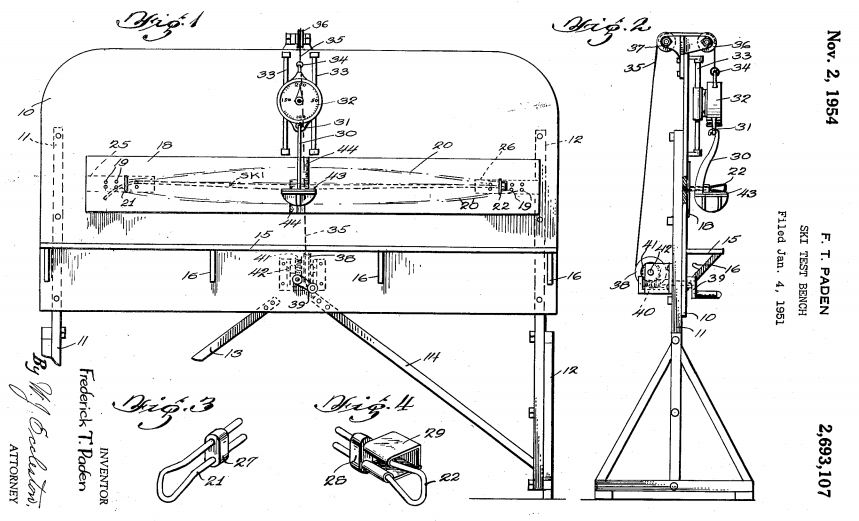
\includegraphics[width=1\textwidth]{figures/earlytb.png}
    \caption{Illustrating the concept of a test bench. Figure from \url{https://patents.google.com/patent/US2693107A/}}
    \label{fig:earlytb}
\end{figure}

The performance of a cross-country skier is highly dependent on the performance and quality of the skis. The ski's performance is determined by several mechanical properties such as the camber height and stiffness. These characteristics will be explained in detail later in this thesis. Another vital factor for the performance of the ski is the wax applied under the skis, both the grip wax to make the ski grip and the gliding wax to make the ski glide. However, it is often claimed that the performance of the skis themselves are roughly 80\% of the total performance, while the remaining approximately 20\% is influenced by the skier and service personnel \citep{ronbeck_vikander_2007,ronbeck_2001}. Grinding of the ski sole is roughly 10\% and the waxing also only 10\%. 

Finding the best skis is a challenge. Skis are chosen by the athletes and the experts together to find the best fit for the athlete. Great resources and time are being spent on manually selecting a large pool of skis for testing in the field. To the author's knowledge, the skis are hand-picked from the manufacturers by experts with intuition and experience. The skis are then stored in a pool of skis for further testing. The manual selection can indicate that the differences in each ski selected are prone to human error in terms of subjective selection. Furthermore, a quantitative way of choosing skis can further improve the ski selection phase by performing objective measurements and selection.

Older methods of testing mechanical properties in materials were done by applying force to the middle of a structure. A measurement device, shown in Figure \ref{fig:earlytb} was typically used to investigate the elasticity of structures like aircraft wings or skis. The concept was to apply forces to the center of the structure, to determine deflection or stress.
Companies like \textit{Skiselector} \ref{subsec:skiselector} and \textit{Gear West Signature Flex Tester} \ref{subsec:gwsft} have developed measurement devices with similar concepts, with focus on measuring the height of the camber and stiffness when applying an external force on the ski. By measuring and collecting mechanical properties, these measurement systems can give each ski a span curve profile used for matching similar skis.

\subsection{Body Weights and Loading Weights}
\label{subsec:bw}
When collecting mechanical properties during measuring of skis, it is necessary to load the ski with the correct weight for the matching ski-phase. These ski phases are the kick phase and the glide phase. Finding the gripping zone, and extracting mechanical properties, the weight of the skier is loaded. The full body weight (FBW) of the skier is loaded to find grip zones. For different snow conditions in terms of warm-, zero- or cold-weather $(\SI{2}{\celsius}> \SI{0}{\celsius} >\SI{-3}{\celsius})$,  the amount of contact from the grip zone during kick-phase is determined by the stiffness of the ski.
During the gliding phase, the skier balances the weight equally onto both skis to avoid the gripping wax from getting contact with the surface. For this phase, the weight loaded on the ski is defined to be the skiers half body weight (HBW).
These weights represent the loads applied on the ski for collecting the mechanical properties of the ski, during kick phase and gliding phase. The binding point (BP), is the point on the ski where the shoe tip attaches to the ski binding and is the reference point of where the force is applied, either at the binding point directly, offset towards or away from the heel point of the binding. Typically, during the kick-phase, the skier wants to apply all force at the binding point for increased contact on the surface. When investigating the skis quality and ability to glide, it is necessary to analyze the mechanical properties of the ski at the skiers half body weight.

\section{Mechanical properties}
\label{sec:mechanicalproperties}
A cross country ski has many mechanical properties. The mechanical properties also referred to as the characteristics, are essential when describing and measuring the quality of a ski. These details are the arch, stiffness, and how the weight distributes along the ski, where the latter is the pressure distribution. Choosing skis with mechanical properties matching the weather conditions is the most important way of finding the right skis. Felix Breitschädel published several papers on different aspects of how the gliding speeds and overall performance can be improved by using skis with different mechanical properties and sole structures.
Furthermore, his thesis leads to the development of a new low-cost inertial measurement unit(IMU)-based sensor to investigate camber height and heat maps where the ski presses on the surface. This measurement unit produced reasonable estimates to distinguish between good and bad skis. The mechanical properties used imaging of the sole to generate heat maps of the pressure areas \citep{breitschadel_technical_2014}. 
\newline

\subsection{Span curve}
\label{subsec:spancurve}
The span curve is the curvature of a ski profile that represents the camber height along the longitudinal length of the ski at HBW or FBW. As shown in Figure \ref{fig:spancurve}, the force is applied at the balance point. The span curve is extracted by pushing the ski down and measuring the height from the surface to the ski sole. The span curve is further used to determine the flex and stiffness of the ski and is essential for finding matching cross-country skis and is also related to camber height \ref{subsec:camberheight}.

\begin{figure}
    \centering
    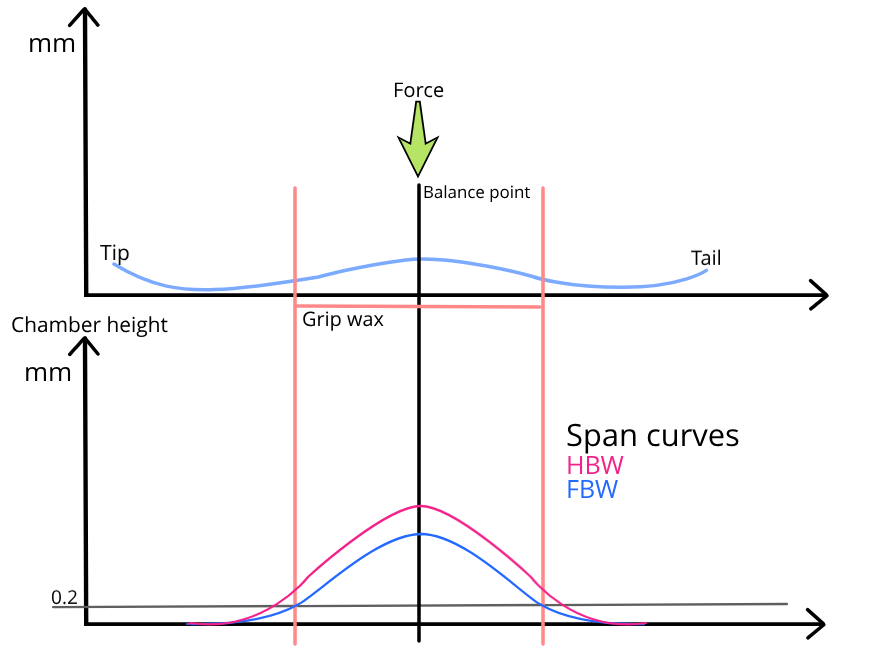
\includegraphics[width=1\textwidth]{figures/spancurve.png}
    \caption{An illustration of the span curves with HBW and FBW.}
    \label{fig:spancurve}
\end{figure}

\subsection{Camber height}
\label{subsec:camberheight}
The mechanical property camber height is described as the height from a flat surface to the sole of the ski.
The purpose of looking at the camber height at FBW and HBW is to find the contact area for gripping wax to be applied. Typically, the skis are marked on the side of the ski when the camber height is $0.2mm$ at both sides of the binding. Preferably, this height is when FBW is loaded. Contact is defined as the camber height at $0.05mm$ \citep{breitschadel_technical_2014}. Marking the waxing zone at FBW results in the gripping wax not establishing contact with the snow during the gliding phase (HBW).  The purpose of the marks is to define the gripping area on the sole, so the gripping wax establishes contact with the surface during kick phase  \citep{breitschadel_variation_2012}.
Furthermore, the definition of camber response is the change of camber height in $mm$ per $N$. The camber response is found by loading the BP from 0.5 to 1 times the BW. The camber response is used to calculate the stiffness of the ski \citep{breitschadel_technical_2014}.

\subsection{Stiffness}
\label{subsec:stiffness}
Stiffness is the skis ability to withold forces. Also, it is related to the stiffness at FBW and HBW when selecting a matching pair of skis. The purpose of this mechanical property is to estimate the stiffness of a ski when the body weights are loaded. Stiffness contributes to giving the wanted camber heights and span curve profiles for individual users concerning their body weight and is essential when finding a pair of matching skis for the different weather conditions. The stiffness, $k$, is the relation between the skier's body weight and the camber response of the ski.

\subsection{Pressure Distribution}
\label{subsec:pressuredistribution}
Pressure distribution is a mechanical property that describes the transferred forces to the surface along the longitudinal length of the cross-country ski. Pressure distribution characteristics are obtained by measuring the forces on the surface were the ski presses down. The purpose of measuring the forces at specific points is to find hot spots of forces on the surface which contributes to frictional melting (Section \ref{subsec:skisandsnow}), and how the ski structure distributes weight along the surface from the ski. Further on, fluctuation in the ski structure under stress indicates the ski quality in terms of twisting and even weight transfer along the latitudinal length of the ski. The pressure distribution can work as an additional property for finding a suited match of skis for an athlete. \cite{nilsson2013} researched how the force distribution changed when the loading point (center of mass) moved backward from the original BP position. This investigation can also confirm the interest of looking at the ski characteristics when a skier transitions from a kicking-phase to a gliding phase, where the skier shifts the body weight over to the heel in a resting position.

\begin{figure}
    \centering
    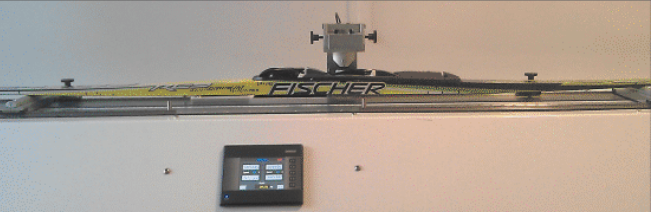
\includegraphics[width=1\textwidth]{figures/testbench.png}
    \caption{Ski test bench developed by Felix Breitschädel. Figure from \citep{breitschadel_technical_2014}}
    \label{fig:tbfelix}
\end{figure}

\section{What makes a ski glide?}
\label{sec:skiglide}
A ski gliding is when positive forces exceed the negative forces working on a skier (Section \ref{subsec:forces}). Positive gravity forces are generated either from going downhill or during kick-phase, resulting in gliding speeds. Overcoming the negative forces are essential for the performance of the skier. A ski slipping or gliding on the snow surface is dependant on the amount of friction between the ski sole and the surface. The friction determines the amount of frictional melting that occurs on the ski sole and generates a thin layer of water film, which decreases the friction. Snow and ice structures determine the amount of water film and friction that is needed. Different characteristics of the snow and snow crystals are not the aim of this study. Detailed characteristics on snow types and snow crystals were researched by \cite{ColbeckSC1986}, and is to the author's knowledge the most recognized and used classification scale for snow. Nevertheless, an understanding of how the forces are affecting the skier's total performance is necessary to investigate.

\subsection{Snow and Ice friction}
\label{subsec:skisandsnow}
Friction between a ski sole and snow or ice surface is highly dependant on; weather, temperature and snow conditions. Factors like the ski characteristics contribute to overcoming the negative forces and the delicate balance between friction and water film. A water film is a thin layer of water gathered up on the ski sole during skiing and is determined by the friction coefficient $\mu$ between the ski sole and the surface. This layer is a result of snow or ice melting due to frictional melting and works as lubrication for improved gliding speeds. The change in friction coefficient was already researched in the mid-nineteenth century by \citep{bowden1939mechanism}. They found that the friction coefficient decreased when the water film is introduced to the polyethylene sole surface \citep{bowden1939mechanism}.
Furthermore, a conclusion was derived that the friction was also related to temperature. Bowden and Hughes found that a decrease in temperature would increase the static friction, indicating lower friction in higher temperatures. 
When sliding speeds are noticeable, the friction decreases and approach a lower value with increasing speeds due to a localized surface melting produced by frictional melting \citep{bowden1953friction}.
A thicker water film is not always the best case for any weather condition. When the water film accumulated exceeds a threshold, and the water film generates drag, which results in reduced gliding speeds. 
More detailed research on the relation between the contact area with the surface and the water film thickness was conducted by \cite{baurle2006sliding}. The increased contact area with the surface with growing water film thickness is illustrated in Figure \ref{fig:waterfilm}. 
As friction is affected by the gravitational forces as well as the accumulated negative forces on the cross-country skier, it is in our best interest to investigate these for understanding which skis characteristics that contributes to better gliding speeds.
\begin{figure}[!htb]
     \centering
     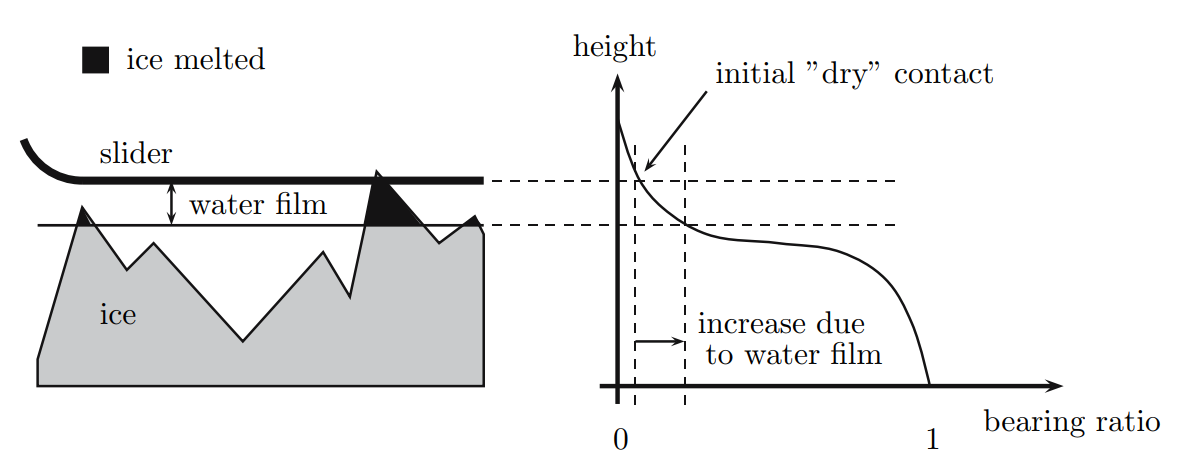
\includegraphics[width=0.99\textwidth]{figures/waterfilm.png}
     \caption{Relation between the water-film thickness and the real contact area (bearing ratio). Melting of ice corresponds to a slicing off and leads to the growth of existing contact and the formation of new contacts. Figure from \citep{baurle2006sliding}}
     \label{fig:waterfilm}
\end{figure}

\subsection{Forces working on the skier}
\label{subsec:forces}
In cross-country skiing, the forces illustrated in Figure \ref{fig:glidingforces} are propulsive forces generated through the skier's activity using a combination of poles and kicking and negative forces such as air resistance, drag, and friction. The objective of cross-country skiing is to overcome the negative forces affecting the skier. The forces acting on a skier in a gliding scenario is illustrated in Figure \ref{fig:glidingforces}. An explanation of the model was given thoroughly in \citep{breitschadel_technical_2014}.

According to Newton's \nth{2} Law, the forces in the direction of motion (x) are equal to the skier's mass, \textit{m}, times the acceleration, \textit{a}:
\begin{equation}\label{eqn:newtion2nd}
    \sum F_x = ma
\end{equation}

The skier's propulsion is affected by force ($F$) while gliding, which is the mass ($m$) times the gravity ($g$) on an inclined surface:
\begin{equation}
    F_D = F \sin\alpha = mg\sin\alpha
\end{equation}

The negative forces working against a skier's propulsive forces are air resistance ($F_{air}$) and, the frictional forces working between the snow or ice surface and the ski sole ($F_f$). The total sum of forces become:
\begin{equation}
    F_D - F_{air} - F_f = ma
\end{equation}

The friction coefficient ($\mu$) is defined as the resistance force ($F_f$) divided by the downward working force ($F_D$):
\begin{equation}\label{eqn:frictioneq}
    \mu = \frac{F_f}{F_N}
\end{equation}
\begin{figure}
    \centering
    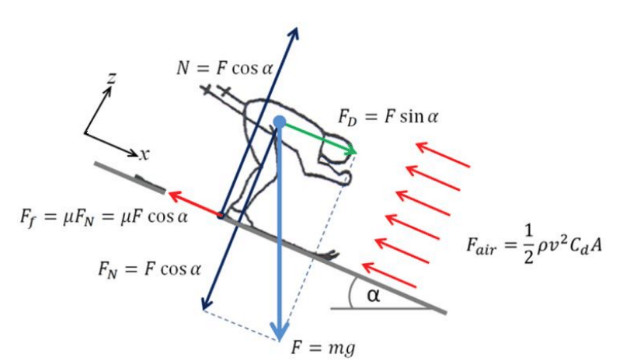
\includegraphics[width=1\textwidth]{figures/forces.png}
    \caption{The forces acting on a skier. Figure from \citep{breitschadel_technical_2014}}
    \label{fig:glidingforces}
\end{figure}
In relation to the pressure distribution \ref{subsec:pressuredistribution}, the static friction coefficient:
\begin{equation}\label{eqn:friction}
    F_{D} = F_f 
\end{equation}

\begin{equation*}\label{eqn:staticfriction}
    mg\sin\alpha = \mu_smg\cos\alpha
\end{equation*}

\begin{equation}\label{eqn:staticfriction2}
    \mu_s = \tan\alpha
\end{equation}
The static friction coefficient ($\mu_s$) is found when the ski is just about to slip ($F_D = F_f$). On the other hand, the kinetic friction coefficient ($\mu_k$) is of interest when the ski is gliding:
\begin{equation}\label{eqn:kineticfriction}
    F_D - F_f = ma
\end{equation}

\begin{equation*}
    mg\sin\alpha - \mu_kmg\cos\alpha = ma
\end{equation*}

\begin{equation*}
    \mu_k = \frac{g\sin\alpha}{g\cos\alpha} - \frac{a}{g\cos\alpha}
\end{equation*}

\begin{equation}\label{eqn:kineticfriction2}
    \mu_k = 
    \begin{cases}
    \mu_s       & \quad \text{if } a = 0\\
    \mu_s - \frac{a}{g\cos\alpha}  & \quad \text{if } a \neq 0
    \end{cases}
\end{equation}
\newline
The adjusting factor when applying the right gliding wax for warm-, zero- or cold-weather conditions, is the amount of kinetic friction between the snow or ice surface and the ski sole. Equation \ref{eqn:kineticfriction2} denotes that the kinetic friction coefficient is equal to the static friction coefficient when the acceleration is zero. At zero acceleration, the skier is in a gliding phase. The gliding wax can either reduce or increase the kinetic friction coefficient to give enough water film for better gliding speeds. For lower temperatures, one will see gliding wax which introduces higher $\mu_k$ for more frictional melting.

\section{Measurement devices}
\label{sec:measurementdevices}
The span curve is an essential descriptor of the mechanical properties of the ski. Several measurement devices have been developed to efficiently and accurately measure the span curve and camber height. The following sections investigate previous research on measurement devices with existing methods for extracting mechanical properties.

\subsection{Eiker måler}
\label{subsec:eiker}
The Eiker ski measurement device was initially developed for the winter Olympics in Lillehammer in 1994 by a Norwegian company called Ski-Test. The idea behind the Eiker-måler was to pair skis with similar flex, also referred to as span curve, and to find a reasonable match to the skier concerning stiffness to weight ratio. Since the start of Ski-test, they have been developing their system with great success, expanding the use to several countries, such as Sweden, Estland, Canada, and the USA to mention a few \citep{eiker_2018}. As instructed by the company, the electrical measurement device loads the ski with a skiers weight to HBW and FBW to mark the gliding zones and kicking zones for application of gliding wax and gripping wax respectively (Figure \ref{fig:eikermåler}).

\begin{figure}
    \centering
    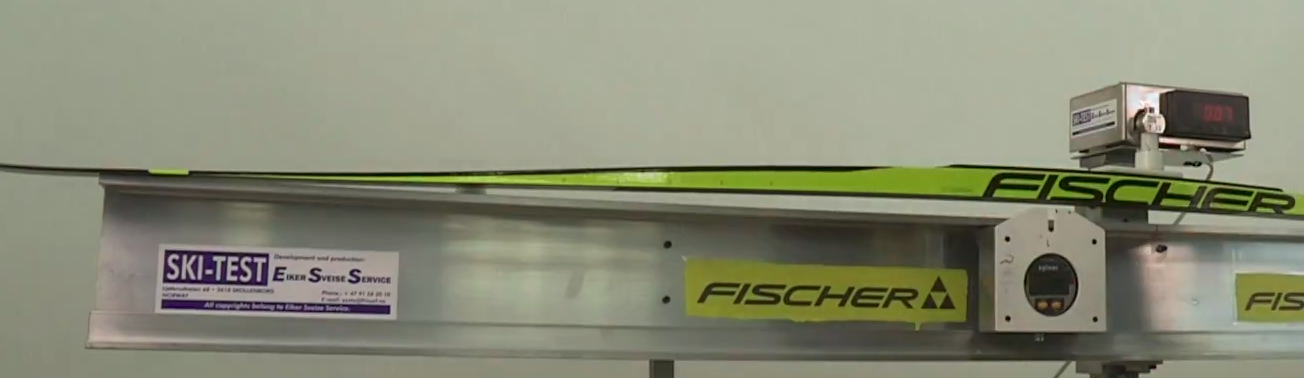
\includegraphics[width=1\textwidth]{figures/eiker.png}
    \caption{An illustration of the "Eiker-måler". Figure from \url{http://www.ski-test.no/instructions/}}
    \label{fig:eikermåler}
\end{figure}

\subsection{SkiSelector}
\label{subsec:skiselector}
The first SkiSelector system was developed for the winter Olympics in Turin in 2006. SkiSelector is a Swedish company, and have increased in popularity since 2006, founded in 2011, the SkiSelector Academy further development of the system. The system delivers a good overview of skis mechanical properties such as grip, stiffness, camber characteristics, and sliding properties. The goal of this system is to give the skier detailed information about the pair of skis and how the skis should be waxed for better grip and glide \citep{skiselector_2018}. The system looks similar to the "Eiker-måler" but instead uses a computer with software to create a profile of each ski measured.

\subsection{IDT Sport - SkiAnalyzer}
\label{subsec:idt}
The SkiAnalyzer from IDT Sport delivers a complete measurement system with different software versions matching the user's experience. The measurements are based on laser technology to measure the camber height and stiffness. Through the software, the system outputs span and stiffness curves. Furthermore, at the end of a measurement, the user can save the measurement data to a database for later use \citep{idt_2018}. The information given by IDT Sport on the SkiAnalyzer (Figure \ref{fig:skianalyzer}) is limited; the system seems to operate with the same precision as SkiSelector and Eiker Måler.

\begin{figure}
    \centering
    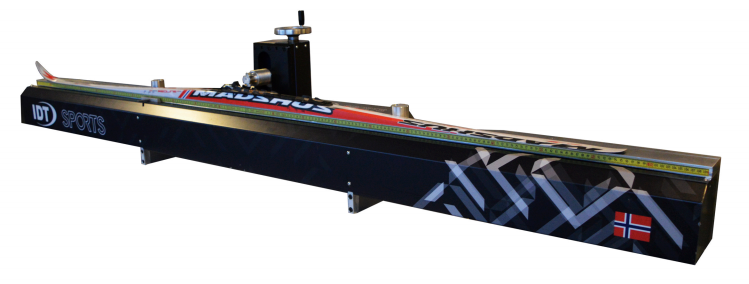
\includegraphics[width=1\textwidth]{figures/skianalyzer.png}
    \caption{An illustration of the SkiAnalyzer from IDT Sport. Figure from \url{https://www.idt.no/sport/produkter/skianalyzer/skianalyzer}}
    \label{fig:skianalyzer}
\end{figure}

\subsection{Gear West Signature Flex Tester}
\label{subsec:gwsft}
Gear West developed the system Ski DNA \citep{skidna_2018}. The system consists of three phases for choosing and measuring cross-country skis, where the first phase is using hands and eyes when squeezing the skis. After the subjective selection, the skier will apply body weight in different positions on the ski. By loading the ski, the ski pocket is found to ensure that the selected skis match each other. The third phase is to put the skis through the Flex Tester measurement bench. The measurement bench is designed to use loading cells to collect pressure distribution data. This data allows the system to check the quality of the flex, weight range, and ideal snow condition for the skis.

\section{Chapter discussion}
In 2008, Bäckström investigated mechanical properties, such as span curve and pressure distribution, and the importance of finding the pressure distribution was further confirmed by Erkillä (1986). These mechanical properties are factors that are affecting the friction, $\mu$, between the skis and snow. Ekström (1980) showed that the friction, $\mu$, decreases with an increased camber value.


\section{Chapter summary}
\label{sec:backgroundconclusion}
Mechanical properties will always be a defining factor between a winning and losing pair of skis. Selecting the right ski for different weather conditions has a significant role in the ski selection phase. A stiffer ski with a short nominal running surface is typically found in classical cross-country skis for warm-weather conditions, giving a steeper increase in camber height at the start of the wax pocket. Warm-weather conditions require a stickier grip wax which introduces a thicker layer of wax. The steep increase in camber height decreases the probability of the gripping wax in the wax pocket and reducing the chance of getting contact with the surface during a gliding phase.
On the contrary, a ski with a more extended nominal running surface is found on classical cross-country skis for cold weather condition. The gripping wax has a dryer consistency, which reduces the overall height of gripping wax applied. The extended nominal contact area will also introduce more frictional melting for generating more water film for better gliding speeds in colder weather conditions.

Based on how the athlete's body weight is loaded on the ski, by for example different pressure points of the foot, varying results in pressure zones onto the ice or snow surface occurs. The thought is that a stiffer structure on the inside of a ski can be countered by a matching weight profile of the foot with extended pressure on the inner side of the foot, resulting in an overall flatter contact of the latitudinal running surface of a ski. With this in mind, it is possible that the friction is more evenly distributed on the surface, resulting in more consistent heat generation and water film due to frictional melting of ice or snow.

The Ski DNA system (Section \ref{subsec:gwsft}), is by far the most interesting. More specifically, the use of loading cells to measure pressure distribution. By using loading cells on prefixed location along with the longitudinal running surface of the ski, we can investigate the forces on each of these points. This investigation could result in pressure distribution profiles for assisting in ski selection. Breitschädel explained that a measurement uncertainty with the Ski Analyzer (Section \ref{subsec:idt}), was affected by the ski running surface. Some sensors on the system could not register contact with the ski, due to the twisting in the skis material.
To the author's knowledge, twisting in the ski structures is a result of deformation of the materials in the ski under production. Finding skis with minimal twisting can result in a more evenly distribution of weight onto ice or snow surface. Twisting can also be considered a property of interest to match the weight transfer from a foot to the ski.
The lack of knowledge on twisting and pressure distribution profiles on classical cross-country skis motivates the development of a measurement device to register both. A measurement device is researched and designed to investigate mechanical properties in classical cross-country skis. In the following sections, a further expansion on existing research and designs lead by multiple sources, such as \cite{ronbeck_2001}, \cite{breitschadel_variation_2012,breitschadel_technical_2014} is further developed.


\chapter{Materials and methods}
\label{chap:materialsandmethods}
\section{Prototyping a measurement device}
\label{sec:measurementdevice}
Early stages of planning and designing a suited measurement device to cover gaps in the research of mechanical properties in cross-country skis. It was first and foremost important to understand what would effect the contact area of the running surface of a ski.
Important factors like stiffness and span curves were already researched thoroughly\citep{breitschadel_variation_2012,breitschadel_technical_2014, backstrom_essential_2008}, and twisting in the structure of the ski was something that would introduce uncertainties in the measurements. 
A further development of the previous mention research project led by Ole Marius Rindal and Jacob Norenberg in \textit{Section \ref{sec:backgroundconclusion}}, had the scope of being something new and a good contribution to the overall research on cross-country skis.
A measurement device in this thesis was developed based on that idea. First concept of this, was to place pressure sensitive films along the ski surface to the register forces and pressure distribution (Figure \ref{fig:earlyprototype}).
The first step in the prototyping a measurement device for this thesis, was to sketch out the basis on what the test bench would need to be able to do:
\begin{itemize}
    \item Measure the weight on multiple points along the ski, also referred to as the pressure distribution.
    \item Reputability in terms of reliable measurements on every occasion of testing.
    \item Detect the start and end of the camber pocket.
    \item Detect differences in a wide selection of skis, to distinguish between good and bad skis.
    \item Detect deflection and twisting in the structure of a ski under load.
\end{itemize}

The first sketch consisted of a polymethyl methacrylate plate (plexiglas) as the bottom surface, enveloping the pressure sensitive films with a top plate of the same kind. The top plate would have drilled out holes directly above the sensors, working as a guide for a piston to transfer weight from the ski, directly on to the sensor (Figure \ref{fig:earlyconcept}).

\begin{figure*}[!b]
    \centering
    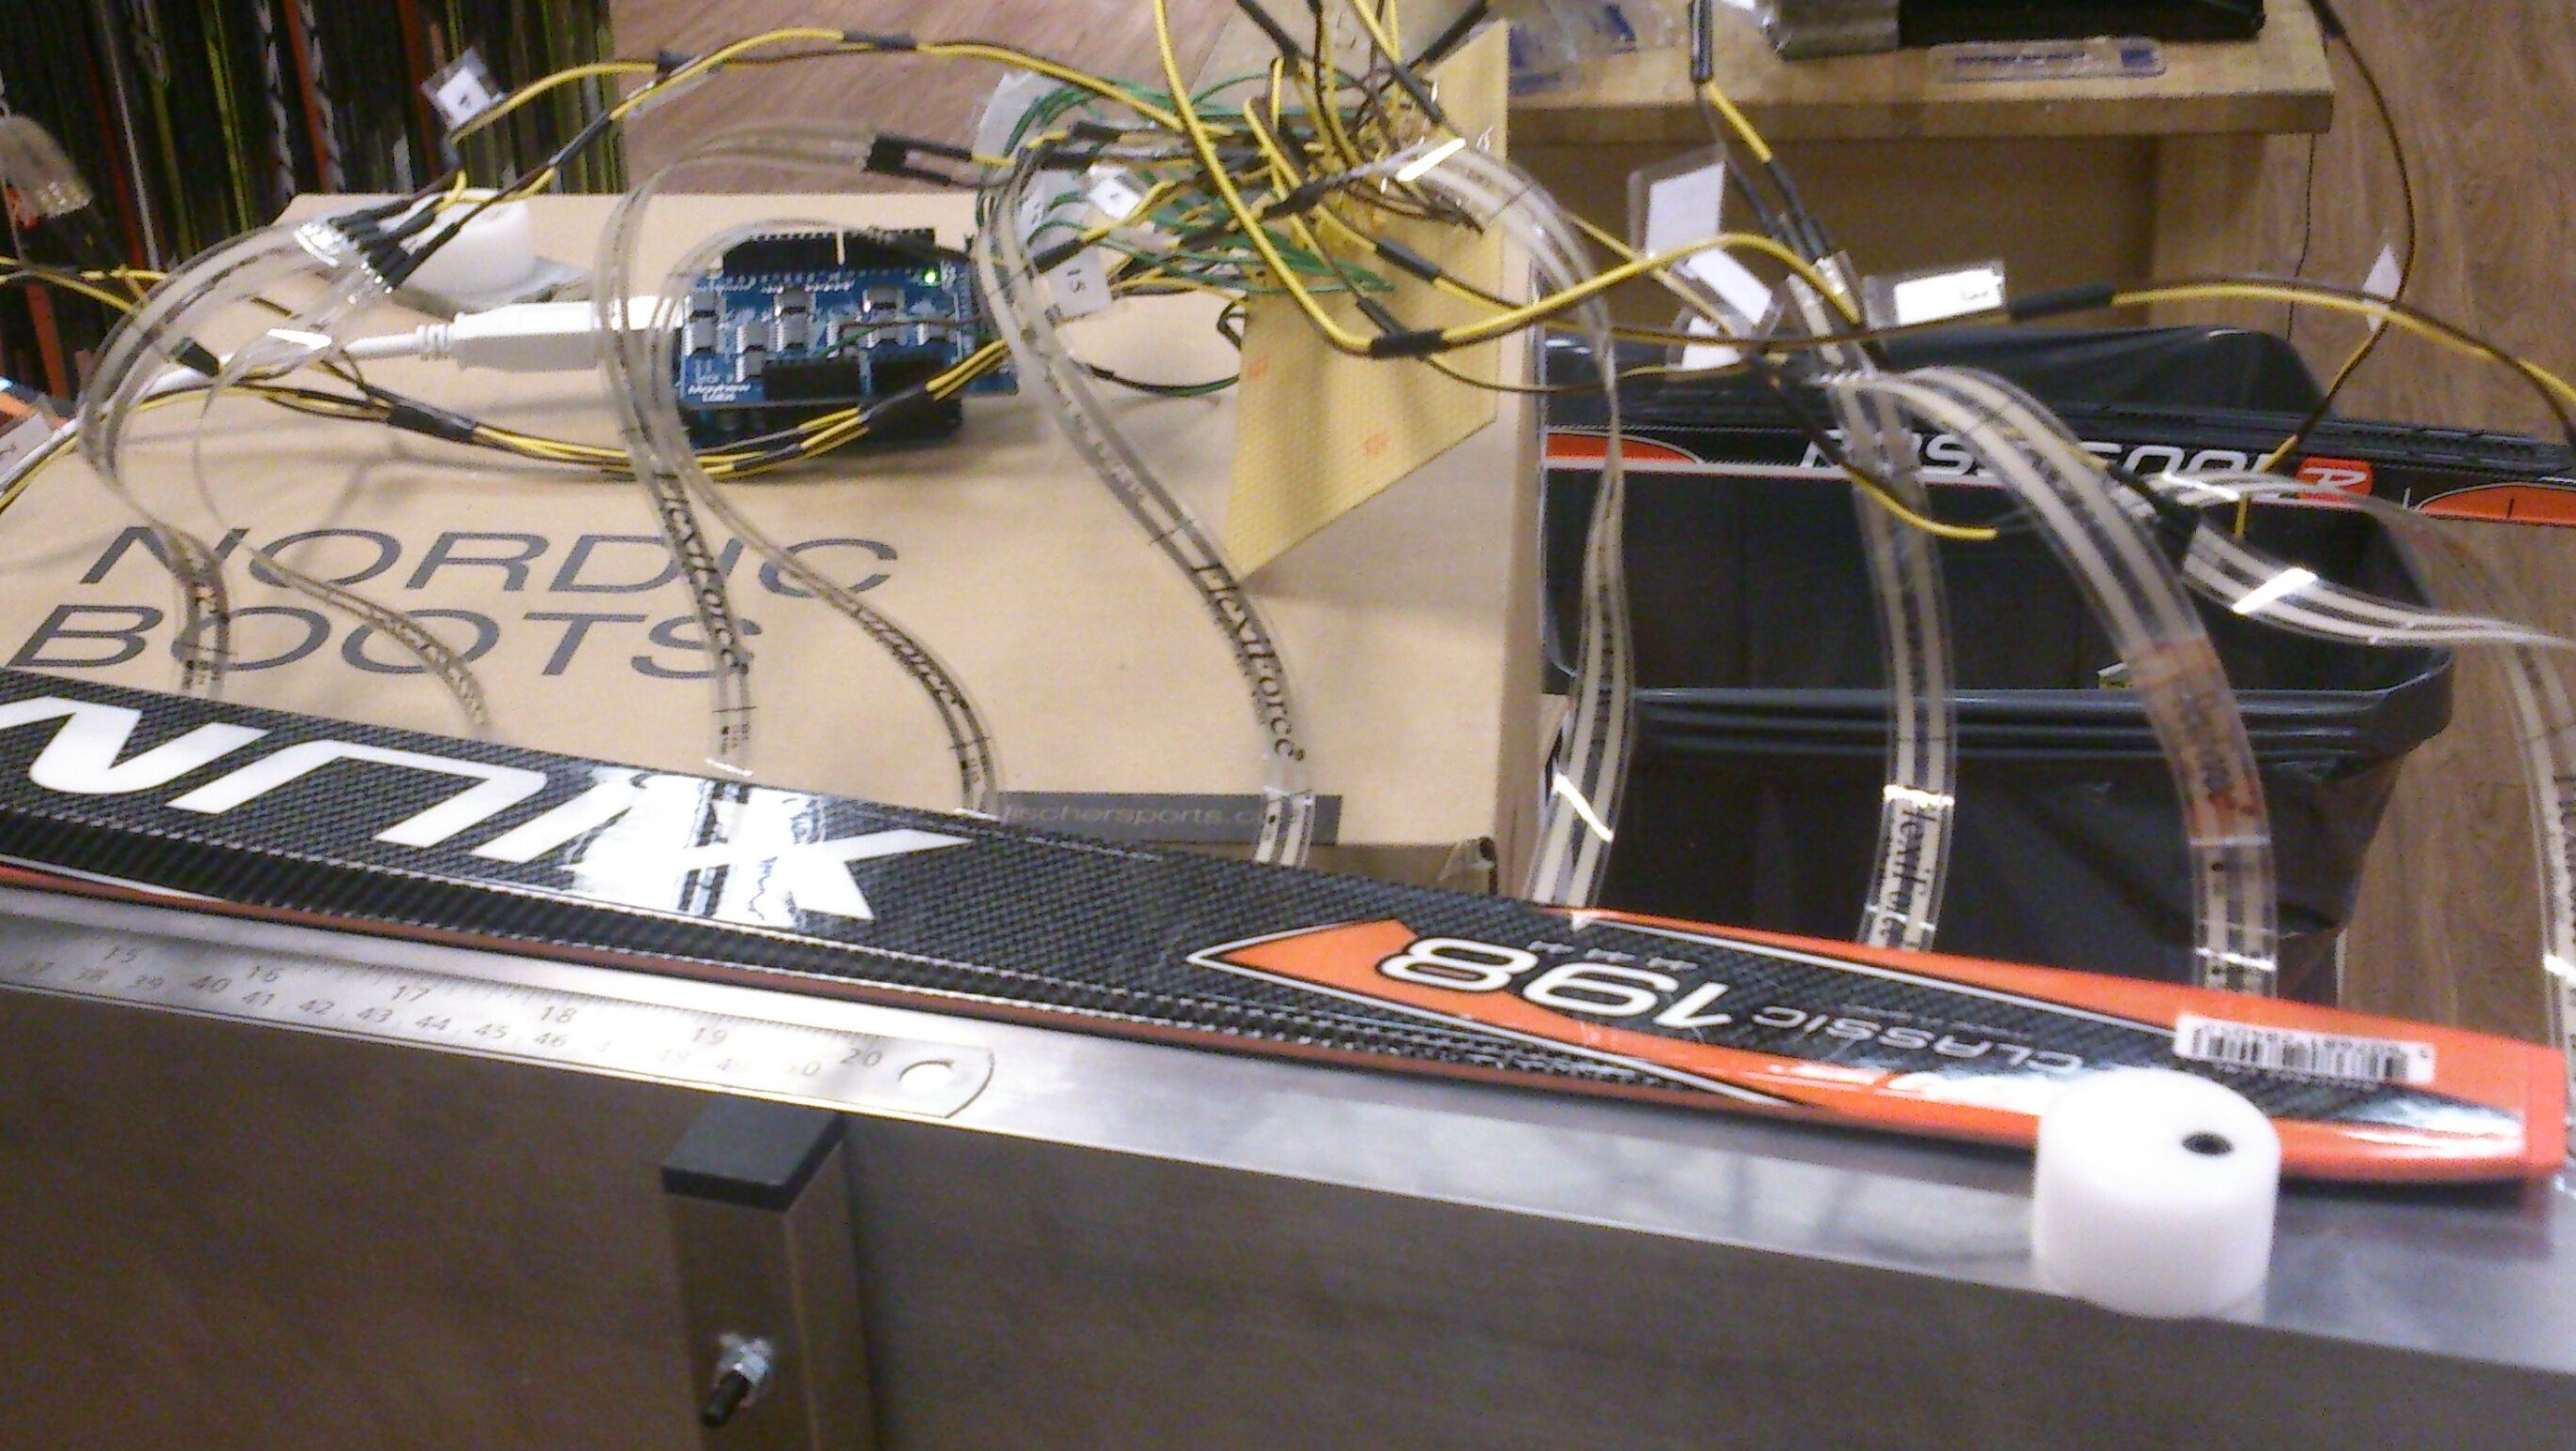
\includegraphics[scale=0.12]{figures/prototype2.jpeg}
    \caption{Photo of student research project led by Ole Marius Rindal and Jacob Norenberg}
    \label{fig:earlyprototype}
\end{figure*}

\begin{figure*}[!b]
    \centering
    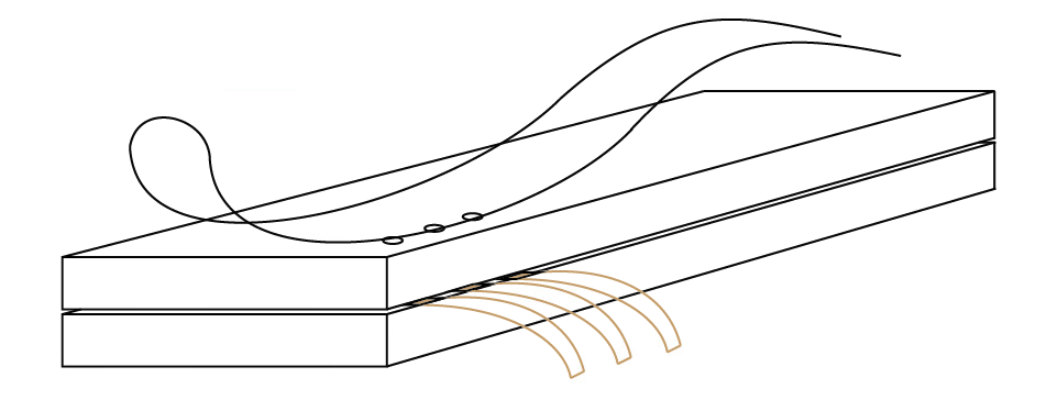
\includegraphics[scale=0.32]{figures/earlyconcept.png}
    \caption{Early concept on sensor placement and structure of a measurement device}
    \label{fig:earlyconcept}
\end{figure*}

To be able to apply force on vertically down on cross-country skis, and also for calibration of the sensors, one would need a digital weight press or manual weights placed on the BP. During the research done on possible ways of applying pressure, we were not able to find an easy solution. Reaching out to alternate resources was necessary.
After consulting with the Instrument Laboratory (I-Lab) at University of Oslo, Department of Physics, we came to a conclusion that the bottom surface had to be more rigid and withstand bending when applying force. I-Lab came up with a solution for applying forces on the ski linearly with a linear guide. This led to a 3D-modelled version of the sketch with the idea of using aluminum for the whole structure, giving the bench more stability and making it stiffer. The 3D-modelled sketch (Figure \ref{fig:3d-modelledsketch} and \ref{fig:3d-modelledsketch_front}) was drawn in AutoDesk Fusion 360 to visualize the concept of the test bench. It then became clear that to be able to produce such a test bench, one would need specialized computer numerical control (CNC) machine for accurate alignment of assembly points where the parts would need to be assembled. Further consultation with I-Lab, led to a collaboration where they were able to draw accurate models of the test bench and manufacture a test bench with the needed specifications for this thesis.
\begin{figure*}
    \centering
    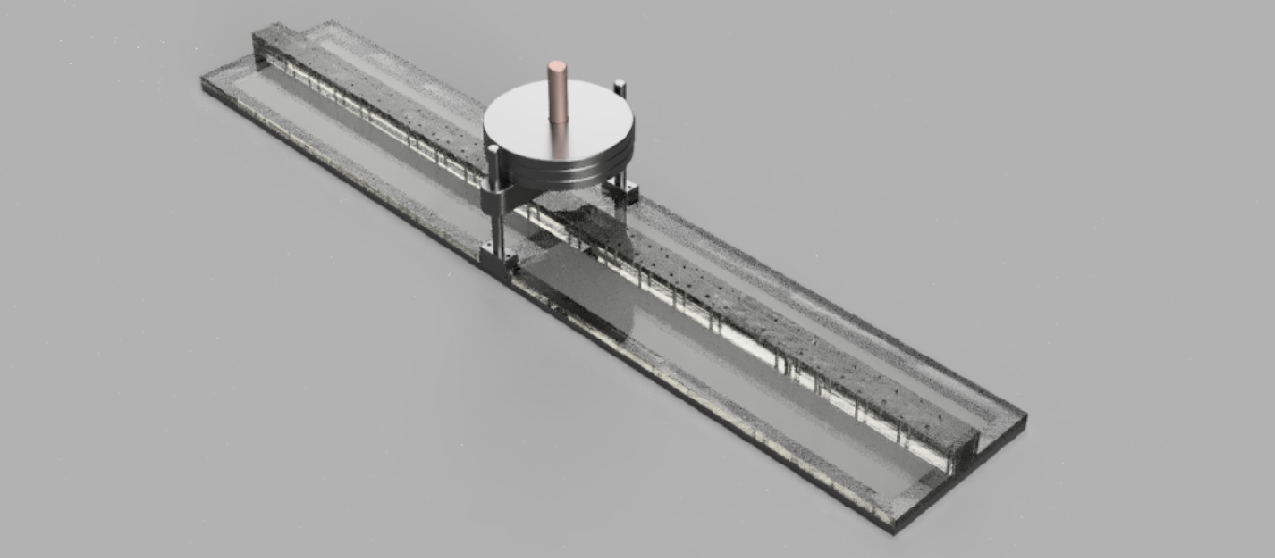
\includegraphics[scale=0.406]{figures/3dmodelledconcept.png}
    \caption{A 3D-model of the concept, drawn in AutoDesk Fusion 360 Student version}
    \label{fig:3d-modelledsketch}
\end{figure*}
\begin{figure*}
    \centering
    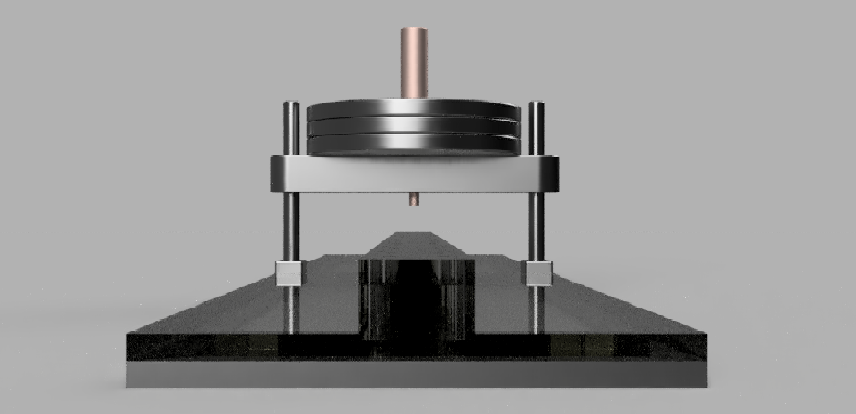
\includegraphics[scale=0.406]{figures/3dmodelledconcept_front.png}
    \caption{A 3D-model of the concept, drawn in AutoDesk Fusion 360 Student version, Front side}
    \label{fig:3d-modelledsketch_front}
\end{figure*}
For the sensors to be place accurately, small pockets were designed for a perfect fit of the sensors circumference. As Figure \ref{fig:3dpockets} show, the pocket holes guiding the sensor with an underlying "puck" (or piston) for a pinching effect on the sensor. This pinching effect was described to give more accurate results in measurements, using pucks on either side of the sensor \citep{vecchi_experimental_2000}. The "pucks" needed to cover at least $80\%$ of the measurement area on the sensor \citep{tekscanA201}. The pockets were placed with a center-to-center distance of $25mm$ along the whole length of the measuring block of $215cm$ containing the sensors. And, with a second row with a center-to-center distance across of $30mm$. This was done for the flexibility of placing and moving the sensors to areas of interest, leaving the empty pockets unused. The linear weight guide was designed to load the weight linearly down on the BP of the ski. With the additional option of a adjustable plate, representing of a foot to adjust the loading point offset from the BP. This was designed with the thought of being able to investigate pressure distribution characteristics at different ski phases, being gliding-phase and kicking-phase.
A locking mechanism was placed at the back end of the measurement block, for the ski to be locked in place centered. This, in combination of the attached adjustable plate at the linear weight guide, would in theory center the ski perfectly on the measurement block. 
\begin{figure*}
    \centering
    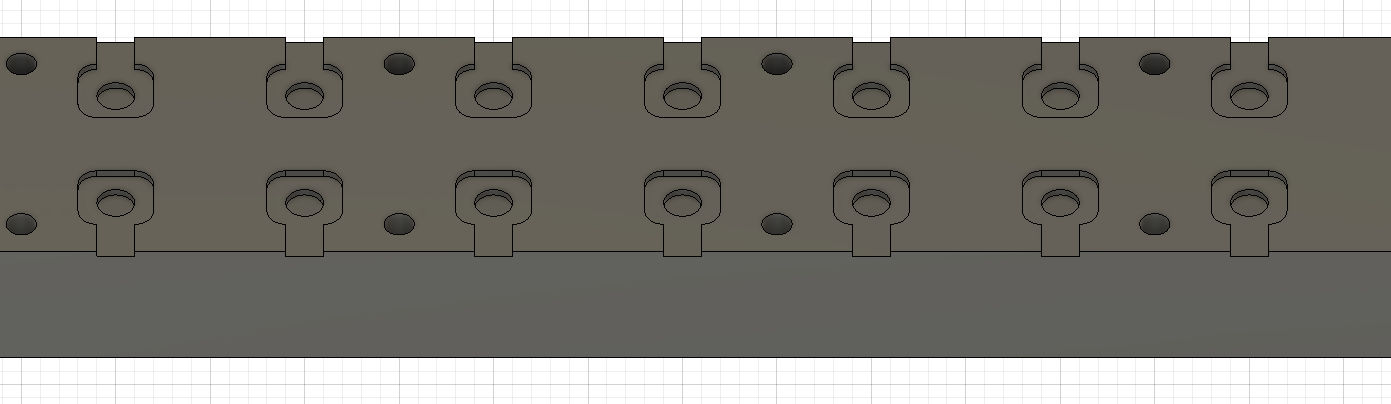
\includegraphics[scale=0.3]{figures/pockets.png}
    \caption{A 3D-model of the pockets for sensor placement}
    \label{fig:3dpockets}
\end{figure*}

The upper part of measurement block have holes of $9mm$ drilled out, for brass pistons or weight transfer pins (WTP) to be placed. As described earlier in this section, this would create a pinching effect on the sensor with the bottom piston part in the pockets. These upper brass pistons of $8mm$, were designed with a detachable plastic cap with threading. These rounded plastic caps would be used for free movement of the ski on top of the WTP.

An additional tool was designed for proper calibration of the sensors. An aluminium beam attached placed on the center between two supporting legs which would rest on the test bench frame. At the end of the beam, a piston matching the hole size of the supporting guides on the measurement block was attached. Weights would then be placed on top of the beam, transferring the loaded weight on to the sensor when calibration of the sensor would be conducted (Section \ref{subsec:calibration}). 

\section{Sensors}
\label{sec:sensors}
\subsection{Pressure sensitive films}
Pressure-sensitive films are simple and thin sensors that are using to measure forces in areas where space is an issue or a requirement. Thin- or thick-films sensors like this can be seen in areas where one would need to register changes in forces to a solid or flexible surface. These force sensing sensors are also referred to as Force Sensing Resistors (FSR). Pressure sensitive films and force sensing resistors are sensors whose resistance decrease with increasing applied force.

\subsubsection{Construction of the sensor}
The name pressure-sensitive film sensor would seem to come from the way it is constructed. The sensor is typically based on five layers. As shown in Figure \ref{fig:sensorconstruction}, the five layers may be the two protective films, which envelopes the sensor as a protective layer. In between, we find the two electrodes enclosing the layer of ink. The electrodes allow electrons to flow through the ink from one electrode to the other.

\begin{figure*}[!b]
    \centering
    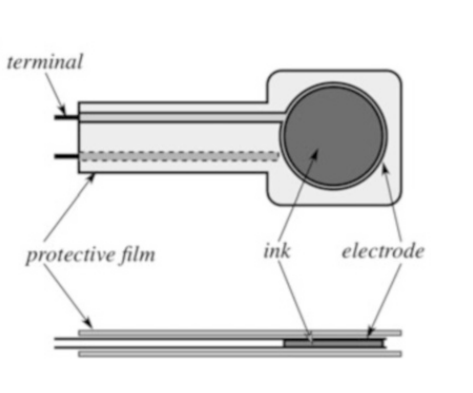
\includegraphics[scale=0.75]{figures/sensorconstruction.png}
    \caption{Composition of thin-film pressure sensor. Figure taken from \cite[p.418]{handbook}}
    \label{fig:sensorconstruction}
\end{figure*}

\subsubsection{Materials}
\label{subsec:materials}
The electrodes can be produced from any conductive material. In terms of producing cheap and reliable sensors, materials like silver can be used. Film materials used as protective layer should be elastic and flexible to allow movement when applying force on the sensor. Flexible material like dielectric Polyester can be used, which also insulates the electrodes. The ink used to conduct electrons between the electrode plates is described to be produced by screen printing piezoresistive ink with a predefined pattern. The ink is printed as thick films having a thickness ranging from 10$\mu m$ to 40$\mu m$. The ink is later dried at 150\textdegree C and then sintered from 700\textdegree C to 900\textdegree C. The sintering makes grains of conductive and insulating oxides bind together and give them cohesion and strength. This results in the ink containing small submicron particles of various metal oxides \citep[10.3, p.418]{handbook}.

\subsubsection{How does the sensor register force?}
When applying force to the sensor, the conductivity increases by increasing connection between the electrodes through three main mechanisms.
The three different mechanisms are conduction, hopping and tunneling.
Based on these, the amount of electrons passing through the ink, increases with more force on the sensor. As shown in Figure \ref{fig:sensorconcept}, conduction is direct contact in the particles of the ink, this happens when the particles are fully connected. Hopping happens when the particles are close enough to allow the electrons to jump. Typically, the jumping effect happens when the distance between the particles are around 10$nm$. The final mechanism is tunneling. This happens when the particles are barely touching (at around 1$nm$) and establishes a path for the electrons \citep[10.3, p.418]{handbook}.

\begin{figure*}[!b]
    \centering
    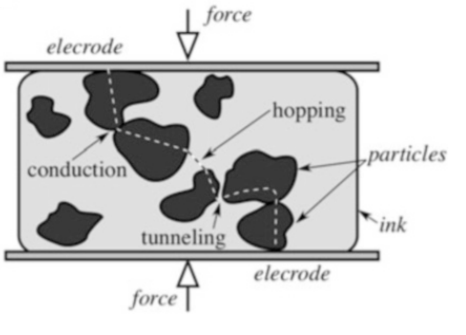
\includegraphics[scale=0.75]{figures/sensorconcept.png}
    \caption{Concept of pressure-sensitive ink. Figure taken from \cite[p.418]{handbook}}
    \label{fig:sensorconcept}
\end{figure*}

\subsubsection{Usage}
The sensor operates in the voltage area of the input voltage of the circuit. This can typically be from $0V$ to $+5V$. By applying force on the sensor, the resistance decreases and conductivity increases. This allows the output voltage to vary, which allows for a simple way of reading and measuring. When the sensor is idle, without load, the sensor is described to have mega-ohms of resistance or infinite impedance. This makes the idle state difficult as a minimum value for calibration. The sensor should be loaded with a small weight, covering around 80\% of the sensor's measuring surface \citep[10.3, p.418]{handbook}. Due to potential noise and spikes in the measurement, one should consider low-pass filtering with a capacitor, this is later tested in Chapter \ref{subsec:capacitor}.
The circuits used are simple voltage dividers or operational amplifier circuits. Where the latter prevents the sensor to draw power directly from the supply voltage. For best results, one should consider different circuits for specific application area.

\subsubsection{Measurement quality}
The pressure-sensitive sensor is known for having linear measurements (the linearity error can typically be $\pm$ 3\%) and has a moderate application difficulty. The measurements do on the other hand have some issues when it comes to measuring over longer periods of time. The ink material need time to reset after a period of measuring. The conductance can increase exponentially and the data is no longer useful. The measurements tend towards non-linear.
Allowing of the ink to settle to ensure consistency in the results is something that is considered when gathering data \citep{vecchi_experimental_2000}.

\subsection{FlexiForce A201 Sensor}
\label{subsec:flexiforce}
The FlexiForce A201 sensor from Tekscan is a pressure sensitive film, constructed of two layers of plastic substrates films like polyester. Each layer consists of a conductive material (silver), which encloses a layer of conductive ink with adhesive, as described in Section \ref{subsec:materials}. The sensing area is defined by a circular pattern of $10mm$, extended to two connectors for reading voltage (Figure \ref{fig:tekscana201}. Tekscan, Inc. offers three variations of the FlexiForce A201 sensor. Low$^1$ 4,4\si{\newton}, Medium$^2$ 111\si{\newton}, and High$^3$ 445\si{\newton}, where the latter can be adjusted to have a sensing area up to 4448\si{\newton} by adjusting the sensitivity in the circuit \citep{tekscanA201}. The idle state of the flexiforce A201, is described to have mega-ohms resistance, making it difficult to read accurate voltages when the sensor is not under load.
\begin{figure*}
    \centering
    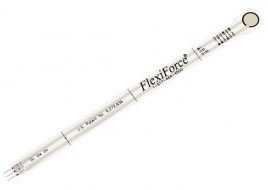
\includegraphics[scale=0.85]{figures/A201.jpg}
    \caption{Force sensing sensor (by Tekscan, Inc.). Figure taken from \textit{https://www.tekscan.com/products-solutions/force-sensors/a201}}
    \label{fig:tekscana201}
\end{figure*}

\subsection{Interlink Force Sensing Resistor}
\label{subsec:interlink}
The Force Sensing Resistor (FSR) from Interlink Electronics is a common device used for sensing changes in force from contact, with an optimized sensitivity for use human touch \citep{interlinkelectronics}. The FSR sensor is a thick-filmed sensor consisting of two conductive layers with interdigitated patterns which is commonly found in heat sensors. The interdigitated layers are deposited on a thermoplastic sheet facing another sheet containing a conductive polyetherimide film. A spacer placed between the sheets allows electrical contact when force is applied \citep{vecchi_experimental_2000}. As the FlexiForce A201 sensor, it is based on a circular construction with a diameter of $14.7 mm$ (Figure \ref{fig:fsr402}). 

\begin{figure*}
    \centering
    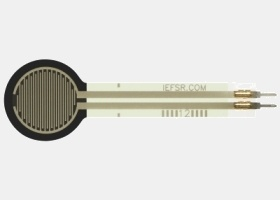
\includegraphics[scale=0.85]{figures/FSR-402.jpg}
    \caption{Force sensing resistor (FSR by Interlink Electronics). Figure taken from \textit{https://www.interlinkelectronics.com/fsr-402}}
    \label{fig:fsr402}
\end{figure*}

\subsection{Calibration of the sensors}
\label{subsec:calibration}
The calibration of the sensor can be done by calibrating the sensor at a minimum- and maximum-weight. Followed by a line fit to create the system response. This works well if we know the linearity of the measurements. If the conductance versus force linearity is known to increase more exponentially, we should consider using knots to section out certain parts of the full scale output. If the measurements should result in non-linearity's, the sensor could be damaged.

\section{Circuits}
\label{sec:circuits}
For measuring the response of a pressure-sensitive film, a circuit should be formed to obtain stable and accurate measurements. Since a sensor draws power from the circuits power source, one will see current drops when applying pressure to the sensor in a regular RC (Resistor-Capacitor) circuit or in a voltage divider. This is where a operational amplifier circuit will come to great benefit.

\subsection{Voltage divider}
A voltage divider is one of the simplest forms of circuits (Figure \ref{fig:voltagedivider}) considered for a pressure-sensitive film. The quality of the measurement result is based on the voltage read from the circuit. The voltage varies when the resistance of the sensor changes due to applied pressure. This voltage is based on the analytic formula in Equation \ref{eq:voltagedivider}. 
\begin{equation}
\label{eq:voltagedivider}
    V_{out} = V_{supply} \cdot \frac{R_1}{R_{flexiforce} + R_1}
\end{equation}
\begin{figure*}[!b]
    \centering
    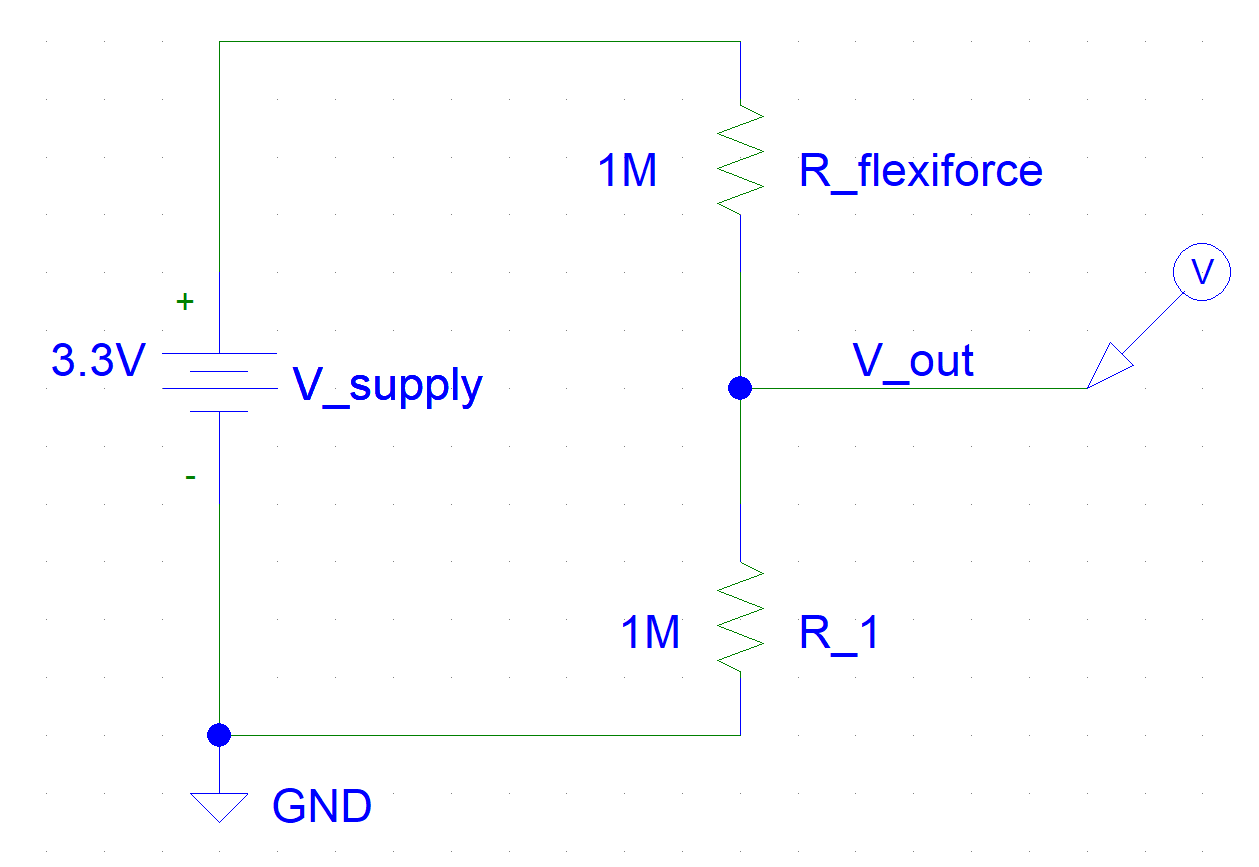
\includegraphics[scale=0.45]{figures/voltage_divider.png}
    \caption{Voltage divider circuit for sensing changes in pressure sensitive films}
    \label{fig:voltagedivider}
\end{figure*}
When applying pressure on the sensor, the resistance decreases, resulting in an increase in voltage in $V_{out}$. This voltage can be calibrated and transformed directly to weight ($Kg$) for the specific sensor in use. One of the benefits of using a voltage divider, is the easy implementation. On the contrary, we can experience more interference in the measured voltage and measurement spike due to the sensor drawing power straight from the power source. !Kg formula

\subsection{Operational amplifier circuits}
\label{subsec:opamps}
Operational amplifiers are 3 terminal devices used to amplify voltages, two inputs and 1-output, with an addition of power connections ($V_{supply}$). These so called OP-amps are described to have infinite input impedance, meaning it has infinite resistance on the two inputs, making current impossible to flow between them. And, zero output impedance. This is the case for ideal Op-amps, where in the real world applications, no Op-amp is perfect and some variations in current and voltage may occur. Operational amplifiers can be connected into two main forms of circuits, the \textit{Inverting operational amplifier circuit} and \textit{Non-inverting operational amplifier circuit}. By leaving the two inputs open, the ideal operational amplifier is defined to be in a "Open-loop"-state, resulting in infinite gain (A) and bandwidth. In real world applications, the gain can be adjusted by increasing or decreasing the feedback- or input-resistance and is a measure of how good a operational amplifier is. The power connectors on the operational amplifier is defined as $V_{supply}$, which decides the operational voltage range of the amplifier. This operational voltage range usually caps at $\pm 15V$, which gives us a upper limit of how much the circuit is able to amplify a signal.

\subsubsection{Inverting Operational amplifier circuit}
The inverting operational amplifier (Figure \ref{fig:invertingopamp}) is based on the characteristics described in Section \ref{subsec:opamps}. It is the version of the Op-amp circuit that connects the feedback to the negative input (negative feedback) of the two available, making the state of the op-amp "closed-loop". This results in an amplified signal with a negative sign, giving an overall reduced amplification. In this case, the pressure sensitive film, is connected as the $R_{in}$ resistor, which allows the output voltage $V_{out}$ to vary from $0V$ to $-V_{supply}$. When applying force to the sensor, resistance decreases and voltage on the output increases (Equation \ref{eq:invopamp_amplifier_vout}).

\begin{equation}
\label{eq:invopamp_amplifier}
    A = \frac{V_{out}}{V_{in}} = - \frac{R_{feedback}}{R_{flexiforce}}
\end{equation}

\begin{equation}
\label{eq:invopamp_amplifier_vout}
    V_{out}= -V_{in} \cdot \frac{R_{feedback}}{R_{flexiforce}}
\end{equation}

\begin{figure*}
    \centering
    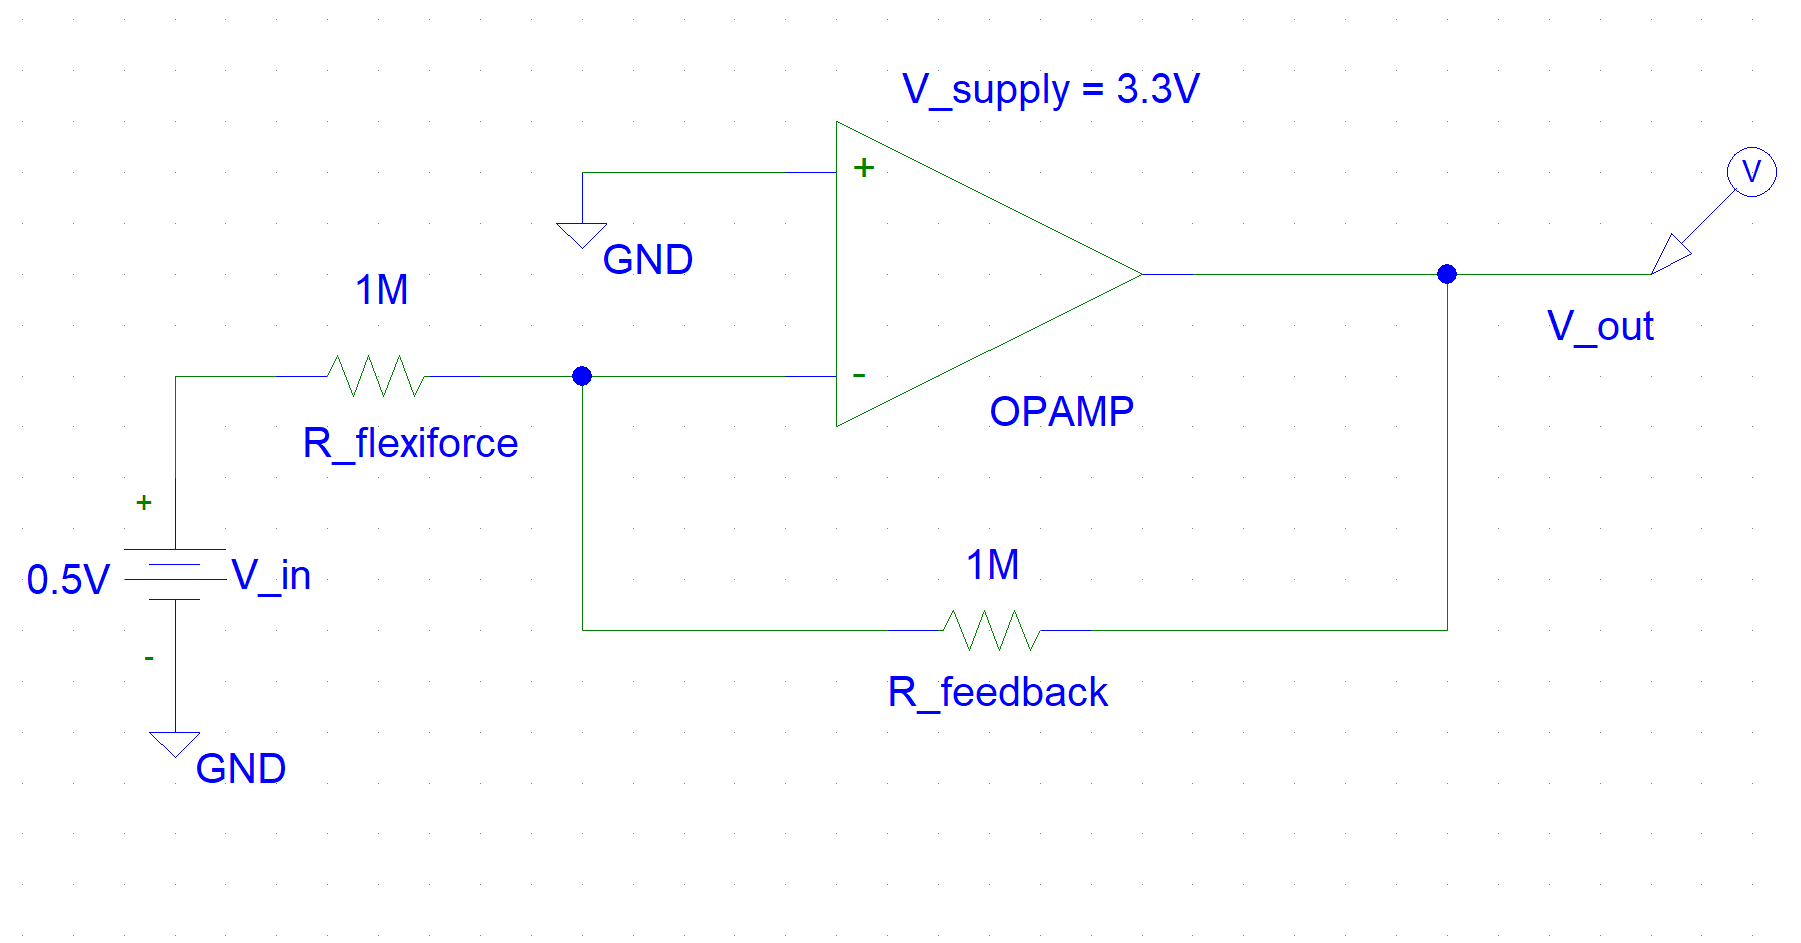
\includegraphics[scale=0.3]{figures/inverting_opamp.png}
    \caption{Inverting operational amplifier circuit for sensing changes in pressure sensitive films (in unity state A=1)}
    \label{fig:invertingopamp}
\end{figure*}


\subsubsection{Non-inverting operational amplifier circuit}
Much like the Inverting operational amplifier, the non-inverting version (positive feedback) connects its feedback to the negative input on the op-amp, but is running voltage input on the positive side. With the addition of feedback running to ground (Figure \ref{fig:noninvertingopamp}). The effect of using a non-inverting operational amplifier circuit is an overall increase in gain compared to the inverting op-amp circuit. Due to the overall increase in amplification, seen from Equation \ref{eq:noninvopamp_amplifier_vout}, one can experience instabilities in the output for lower values of voltage (micro volts).
\begin{equation}
\label{eq:noninvopamp_amplifier}
    A = \frac{V_{out}}{V_{in}} = 1 + \frac{R_{feedback}}{R_{flexiforce}}
\end{equation}

\begin{equation}
\label{eq:noninvopamp_amplifier_vout}
    V_{out} = V_{in}(1 + \frac{R_{feedback}}{R_{flexiforce}})
\end{equation}

\begin{figure*}
    \centering
    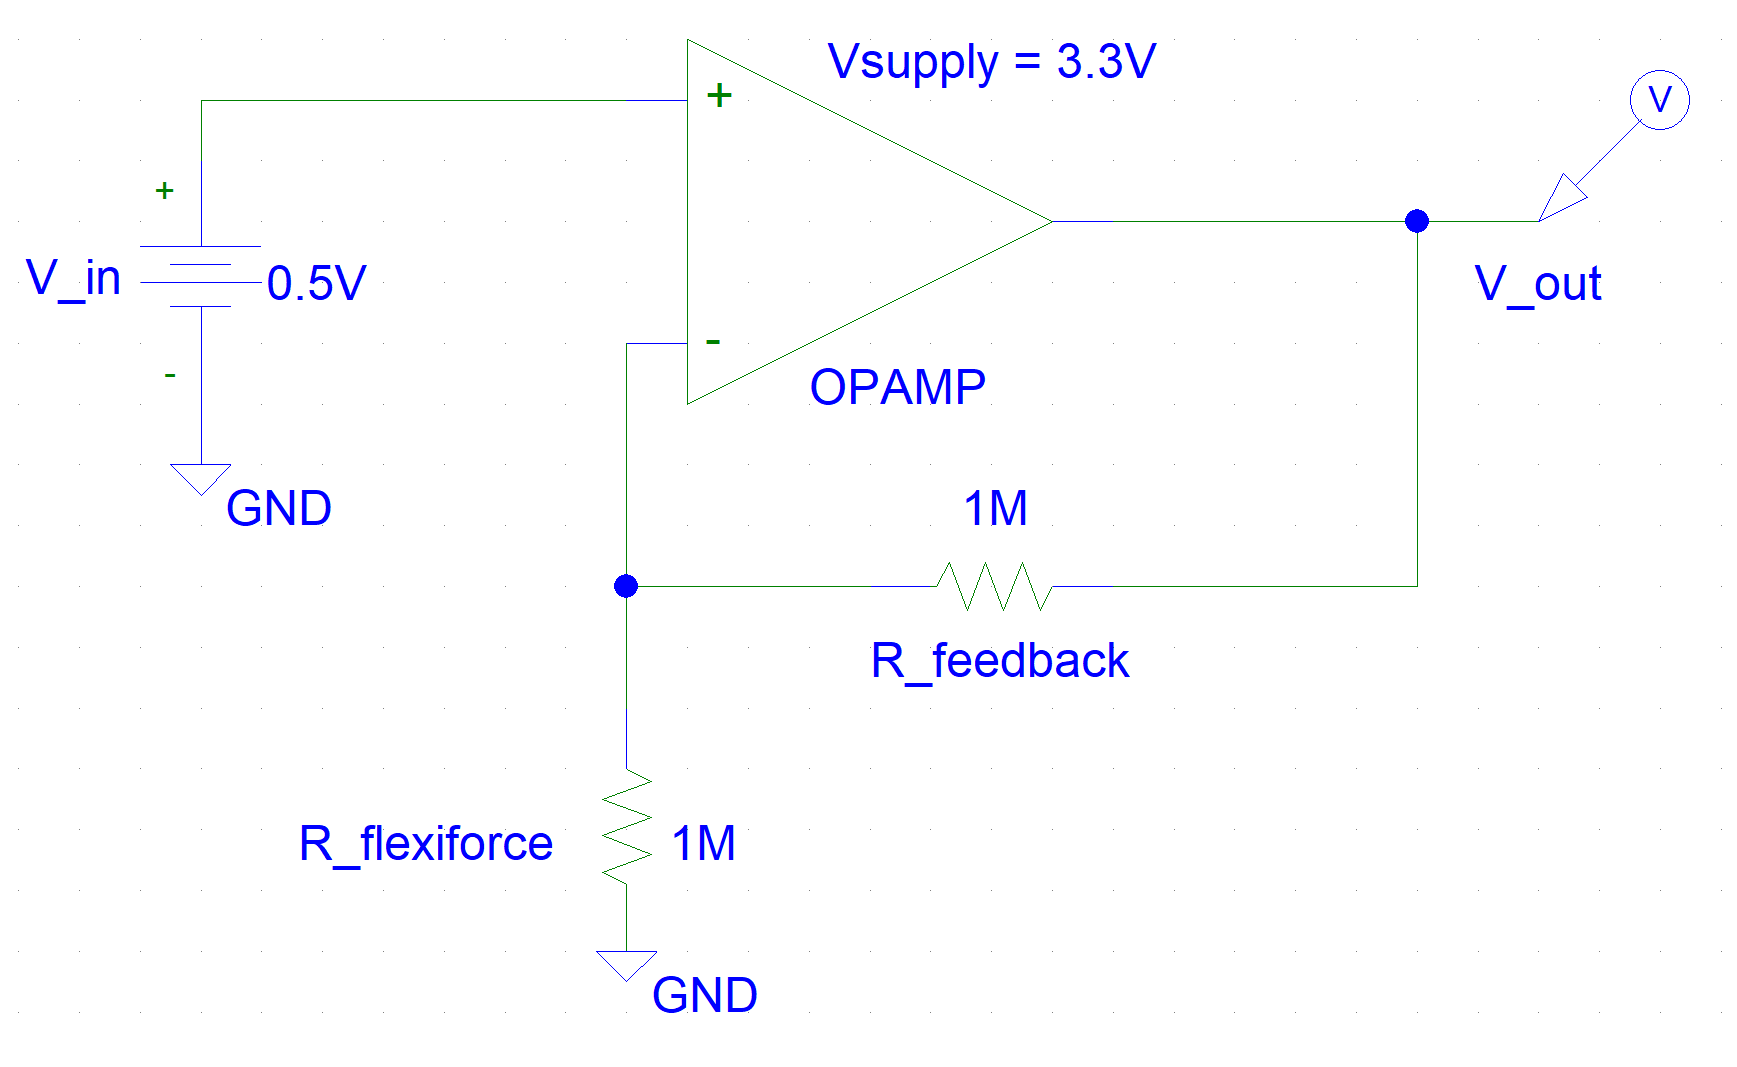
\includegraphics[scale=0.3]{figures/noninverting_opamp.png}
    \caption{Non-inverting operational amplifier circuit for sensing changes in pressure sensitive films}
    \label{fig:noninvertingopamp}
\end{figure*}

\subsection{Implementation of a capacitors}
\label{subsec:capacitor}
When it comes to implementing a analog low-pass filter, a capacitor in parallel with the feedback resistance is implemented in the operational amplifier circuits (Figure \ref{fig:capacitor}) as a first order low-pass filter. One would see this as an option to deal with high frequency spikes in the measurements. The capacitors function in parallel with a resistor, is to filter out higher frequencies, dependent on the size of the capacitor. When the capacitor reaches its cutoff frequency $\omega$, it causes a short in the circuit, leading all frequencies higher than the cutoff frequency to ground or a specified point in the circuit. A larger capacitor will have lower higher cutoff frequency as defined in Equation \ref{eq:cutoff}. By introducing the capacitor, it causes an extra pole in the frequency response of the amplifier circuit, making it more stable. Additionally, introducing capacitors by the power supply and the output of the circuit, additional means of fighting noise in the circuit is introduced.

\begin{equation}
\label{eq:cutoff}
    \omega = \frac{1}{R_{feedback}C_1}
\end{equation}

\begin{figure*}
    \centering
    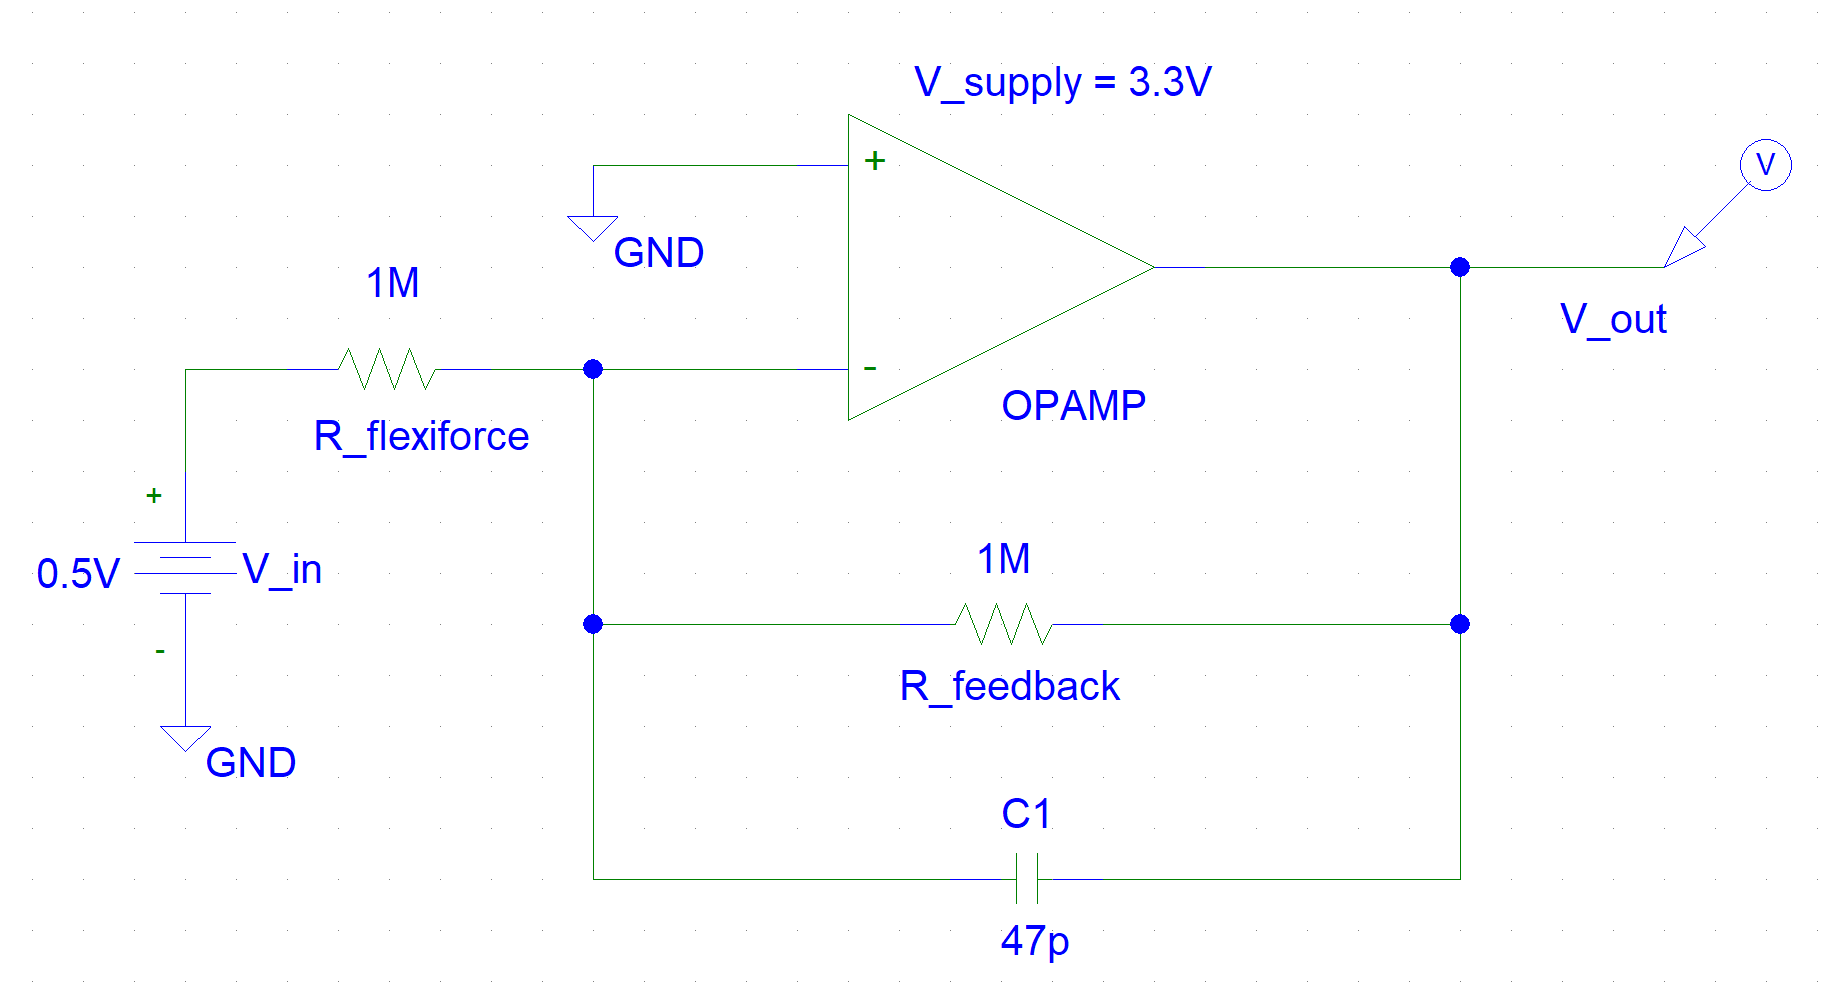
\includegraphics[scale=0.28]{figures/capacitor.png}
    \caption{Inverting operational amplifier circuit with capacitor}
    \label{fig:capacitor}
\end{figure*}


\section{Calibration methods}
Calibration is an essential part of a measurement process and should be done regularly for consistent results. This section explains the concept of calibration why we do it.

\subsection{Modifying the full scale output}
The full scale output (FS) is the relation between input stimulus ($s$) and the output response. It defines the maximum value the system is able to output with given stimulus. Essentially, the full scale output is the measured voltage from the measurement system and can be modified digitally when reading the voltage.
The calibration method can typically be to create a system response based on a statistical line fitting model between a minimum- and maximum-value. For calibration in this thesis, we will see calibration be done with weights in five stages with different weights (also known as calibration knots). This is done by telling the system what weight has been loaded and referring this to the amount of voltage read by the micro controller (Chapter \ref{chap:microcontrollers}).

\subsection{Calibration weights}
For the sensors to be calibrated correctly, we are required to have a absolute scale of weights to refer our voltages to. This can be a certain amount of weights increasing linearly to the appropriate application area. For this thesis, a absolute scale can for example be from 1\si{\kilogram} to 20\si{\kilogram}. 

\section{Chapter results}
\label{sec:chapresults3}
Discussing the results gathered when finding the correct circuit with flexiforce, and calibration results.

\section{Chapter discussion}
In the process of selecting a force sensing sensor, it is required to chose the most suited sensor for the application area. In the research done by Fabrizio Vecchi and his colleagues \citep{vecchi_experimental_2000} on commercial sensors in biomechanics and motorcontrol, sensors like the \textit{Flexiforce A201 \ref{subsec:flexiforce}} and \textit{Force Sensing Resistor \ref{subsec:interlink}} were evaluated. In terms of linearity, time-drift tests and robustness, the Flexiforce sensor presented better results. As mentioned, the application area is what determines the choice of sensor, and for this thesis a sensor is required for handling forces significantly higher than previous research. The Flexiforce sensor in combination with the operational amplifier circuits prove to show similar results in terms of linearity, which is a key factor to obtain consistent results in measurements.

\section{Chapter conclusion}
Sensors and circuits presented in Section \ref{sec:sensors} and \ref{sec:circuits}, the linearity and consistency of measurements were tested and evaluated. Differences were found in terms of noise (measurement spikes and variance), linearity and precision. An operational amplifier circuit was selected reasoned by the requirement of precise measurements and linearity. In combination with the Flexiforce A201 sensor, the system was able to handle the required forces up to 450\si{\newton} (or 45-46\si{\kilogram}). As suggested by Tekscan, Inc., a inverting operational amplifier circuit was chosen.
External and internal noise were handled by implementing a capacitor as a analog low pass filter, which proved to affect on the quality of the sampled data.
\begin{itemize}
    \item \textbf{!! How I calibrated and why}
\end{itemize}

\chapter{Microcontrollers}
\label{chap:microcontrollers}
What a microcontroller is and how to use them.

\section{Raspberry pi}
Pros and cons, operating system, compatibility, ADC, sampling frequency, clock speed and ram.

\section{Arduino UNO}
Pros and cons, operating system, compatibility, ADC, sampling frequency, clock speed and ram.

\section{Arduino UNE}
Pros and cons, operating system, compatibility, ADC, sampling frequency, clock speed and ram.

\section{Discussion}

\section{Chapter conclusion}
Which microcontroller that was chosen and why.


\chapter{Circuits}
\label{chap:circuits}
For measuring the response of a pressure-sensitive film, a circuit should be formed to obtain stable and accurate measurements. A sensor is commonly drawing power from the circuits power source. This can lead to current drops under initial loading of the sensor. This is a common observed phenomena which can introduce inaccuracies in the voltage output. An operational amplifier circuit will come to great benefit when sensors are introduced. The operational amplifier is equipped with an external power source for the sensor to draw power from. More details on the alternative circuits are investigated in the following sections.

\section{Voltage divider}
\label{sec:vd}
A voltage divider is one of the simplest forms of circuits (Figure \ref{fig:voltagedivider}) considered for a pressure-sensitive film. The quality of the measurement result is based on the voltage read from the circuit. The voltage varies when the resistance of the sensor changes due to applied force. This voltage is based on the analytic formula: 
\begin{equation}
\label{eq:voltagedivider}
    V_{out} = V_{supply} \cdot \frac{R_1}{R_{flexiforce} + R_1}
\end{equation}
\begin{figure*}[!b]
    \centering
    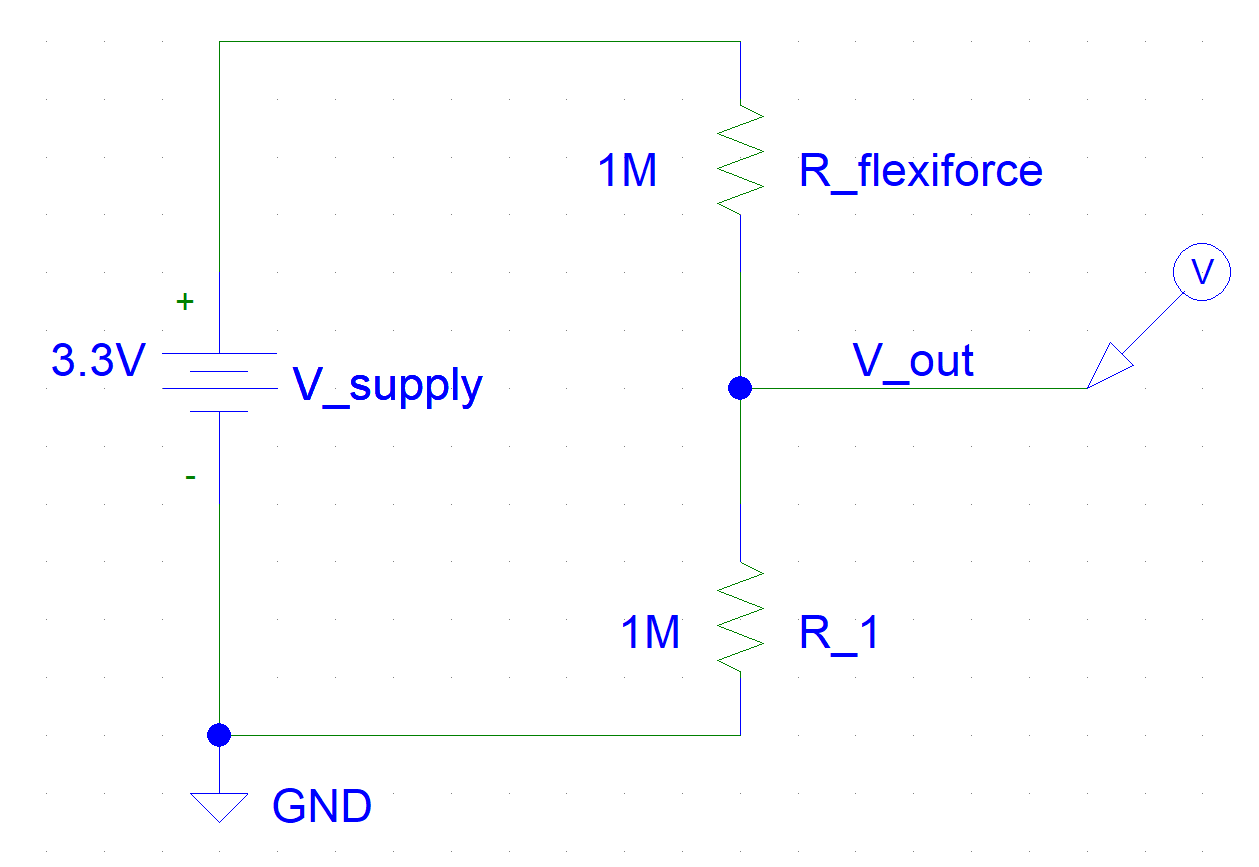
\includegraphics[width=.985\linewidth]{figures/voltage_divider.png}
    \caption{Voltage divider circuit for sensing changes in pressure sensitive films (created in PSpice)}
    \label{fig:voltagedivider}
\end{figure*}
When applying pressure on the sensor, the resistance decreases, resulting in an increase in voltage in $V_{out}$.  One of the benefits of using a voltage divider, is the easy implementation. On the contrary, we can experience more interference in the measured voltage and measurement spike due to the sensor drawing power straight from the power source. !Kg formula

\section{Operational amplifier circuits}
\label{sec:opamps}
Operational amplifiers are 3 terminal devices used to amplify voltages, two inputs and one output, with an addition of two power connections ($V_{supply}$). These so called OP-amps are described to have infinite input impedance, meaning it has infinite resistance on the two inputs, hindering current flow between the inputs and a zero output impedance. This is the case for ideal Op-amps, where in the real world applications, no Op-amp is perfect and some variations in current and voltage may occur. Operational amplifiers can be connected in two main forms of circuits, the \textit{Inverting operational amplifier circuit} and \textit{Non-inverting operational amplifier circuit}. By leaving the two inputs open, the ideal operational amplifier is defined to be in a "Open-loop"-state, resulting in infinite gain (A) and bandwidth. In real world applications, the gain can be adjusted by increasing or decreasing the feedback- or input-resistance and is a measure of how good a operational amplifier is. The power connectors on the operational amplifier is defined as $V_{supply}$, which decides the operational voltage range of the amplifier. This operational voltage range usually caps at $\pm 15V$, which gives us a upper limit of how much the circuit is able to amplify a current to.

\subsection{Inverting Operational amplifier circuit}
\label{subsec:invopamp}
The inverting operational amplifier (Figure \ref{fig:invertingopamp}) is based on the characteristics described in Section \ref{sec:opamps}. This circuit is based on a negative feedback connection of the two inputs available. This results in an amplified signal with a negative sign, giving an overall reduced amplification. In this case, the pressure sensitive film, is connected as the $R_{in}$ resistor, which allows the output voltage $V_{out}$ to vary from $0V$ to $-V_{supply}$, and for a biased input, it can vary from $V_{bias}$ down to $0V$. When applying force to the sensor, resistance decreases and voltage on the output increases (Equation \ref{eq:invopamp_amplifier_vout}).

\begin{equation}
\label{eq:invopamp_amplifier}
    A = \frac{V_{out}}{V_{in}} = - \frac{R_{feedback}}{R_{flexiforce}}
\end{equation}

\begin{equation}
\label{eq:invopamp_amplifier_vout}
    V_{out}= -V_{in} \cdot \frac{R_{feedback}}{R_{flexiforce}}
\end{equation}

\begin{figure*}
    \centering
    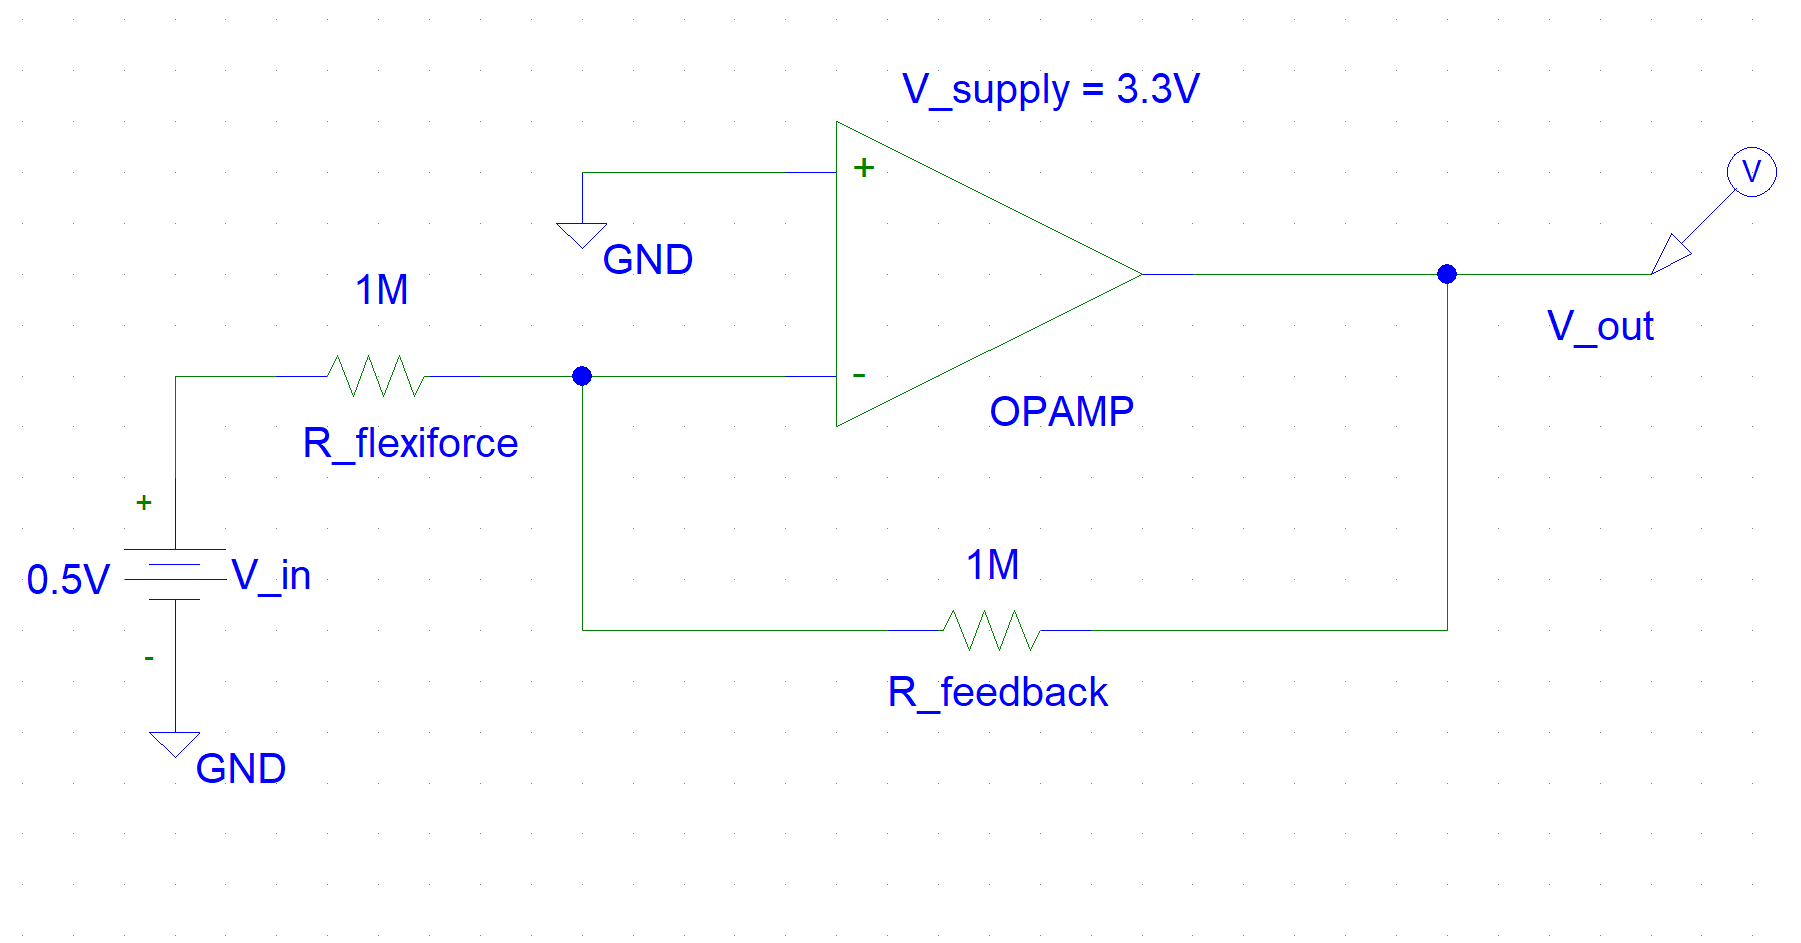
\includegraphics[width=.985\linewidth]{figures/inverting_opamp.png}
    \caption{Inverting operational amplifier circuit for sensing changes in pressure sensitive films, in unity state A=1. (created in PSpice)}
    \label{fig:invertingopamp}
\end{figure*}


\subsection{Non-inverting operational amplifier circuit}
\label{subsec:noninvopamp}
Much like the Inverting operational amplifier, the non-inverting version (positive feedback) connects its feedback to the negative input on the op-amp, but is running voltage input on the positive side. With the addition of feedback running to ground (Figure \ref{fig:noninvertingopamp}). The effect of using a non-inverting operational amplifier circuit is an overall increase in gain compared to the inverting op-amp circuit. Due to the overall increase in amplification, seen from Equation \ref{eq:noninvopamp_amplifier_vout}, one can experience instabilities in the output for lower values of voltage (micro volts).
\begin{equation}
\label{eq:noninvopamp_amplifier}
    A = \frac{V_{out}}{V_{in}} = 1 + \frac{R_{feedback}}{R_{flexiforce}}
\end{equation}

\begin{equation}
\label{eq:noninvopamp_amplifier_vout}
    V_{out} = V_{in}(1 + \frac{R_{feedback}}{R_{flexiforce}})
\end{equation}

\begin{figure*}
    \centering
    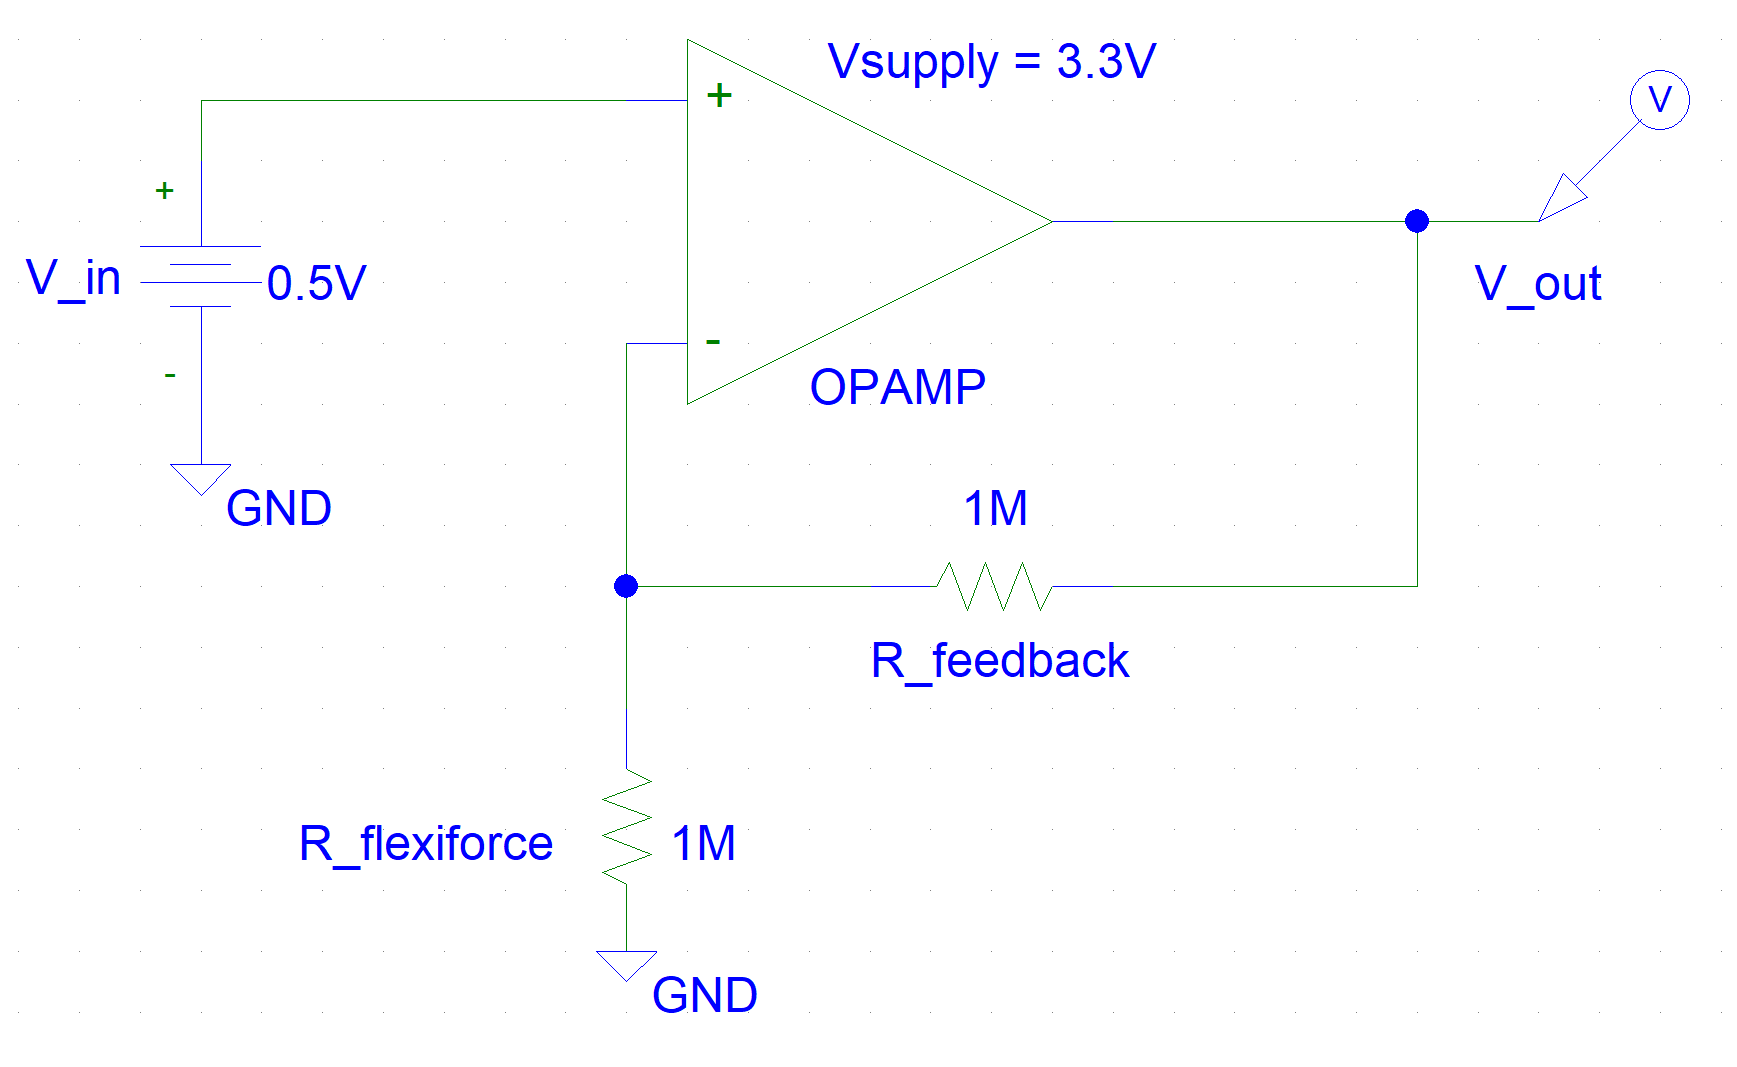
\includegraphics[width=.985\linewidth]{figures/noninverting_opamp.png}
    \caption{Non-inverting operational amplifier circuit for sensing changes in pressure sensitive films (created in PSpice)}
    \label{fig:noninvertingopamp}
\end{figure*}

\section{Implementation of a capacitors}
\label{sec:capacitor}
When it comes to implementing a analog low-pass filter, a capacitor in parallel with the feedback resistance is implemented in the operational amplifier circuits (Figure \ref{fig:capacitor}) as a first order low-pass filter. One would see this as an option to deal with high frequency spikes in the measurements. The capacitors function in parallel with a resistor, is to filter out higher frequencies, dependent on the size of the capacitor. When the capacitor reaches its cutoff frequency $\omega$, it causes a short in the circuit, leading all frequencies higher than the cutoff frequency to ground or a specified point in the circuit. A larger capacitor will have lower higher cutoff frequency as defined in Equation \ref{eq:cutoff}. By introducing the capacitor, it causes an extra pole in the frequency response of the amplifier circuit, making it more stable. Additionally, introducing capacitors by the power supply and the output of the circuit, additional means of fighting noise in the circuit is introduced.

\begin{equation}
\label{eq:cutoff}
    \omega = \frac{1}{R_{feedback}C_1}
\end{equation}

\begin{figure*}
    \centering
    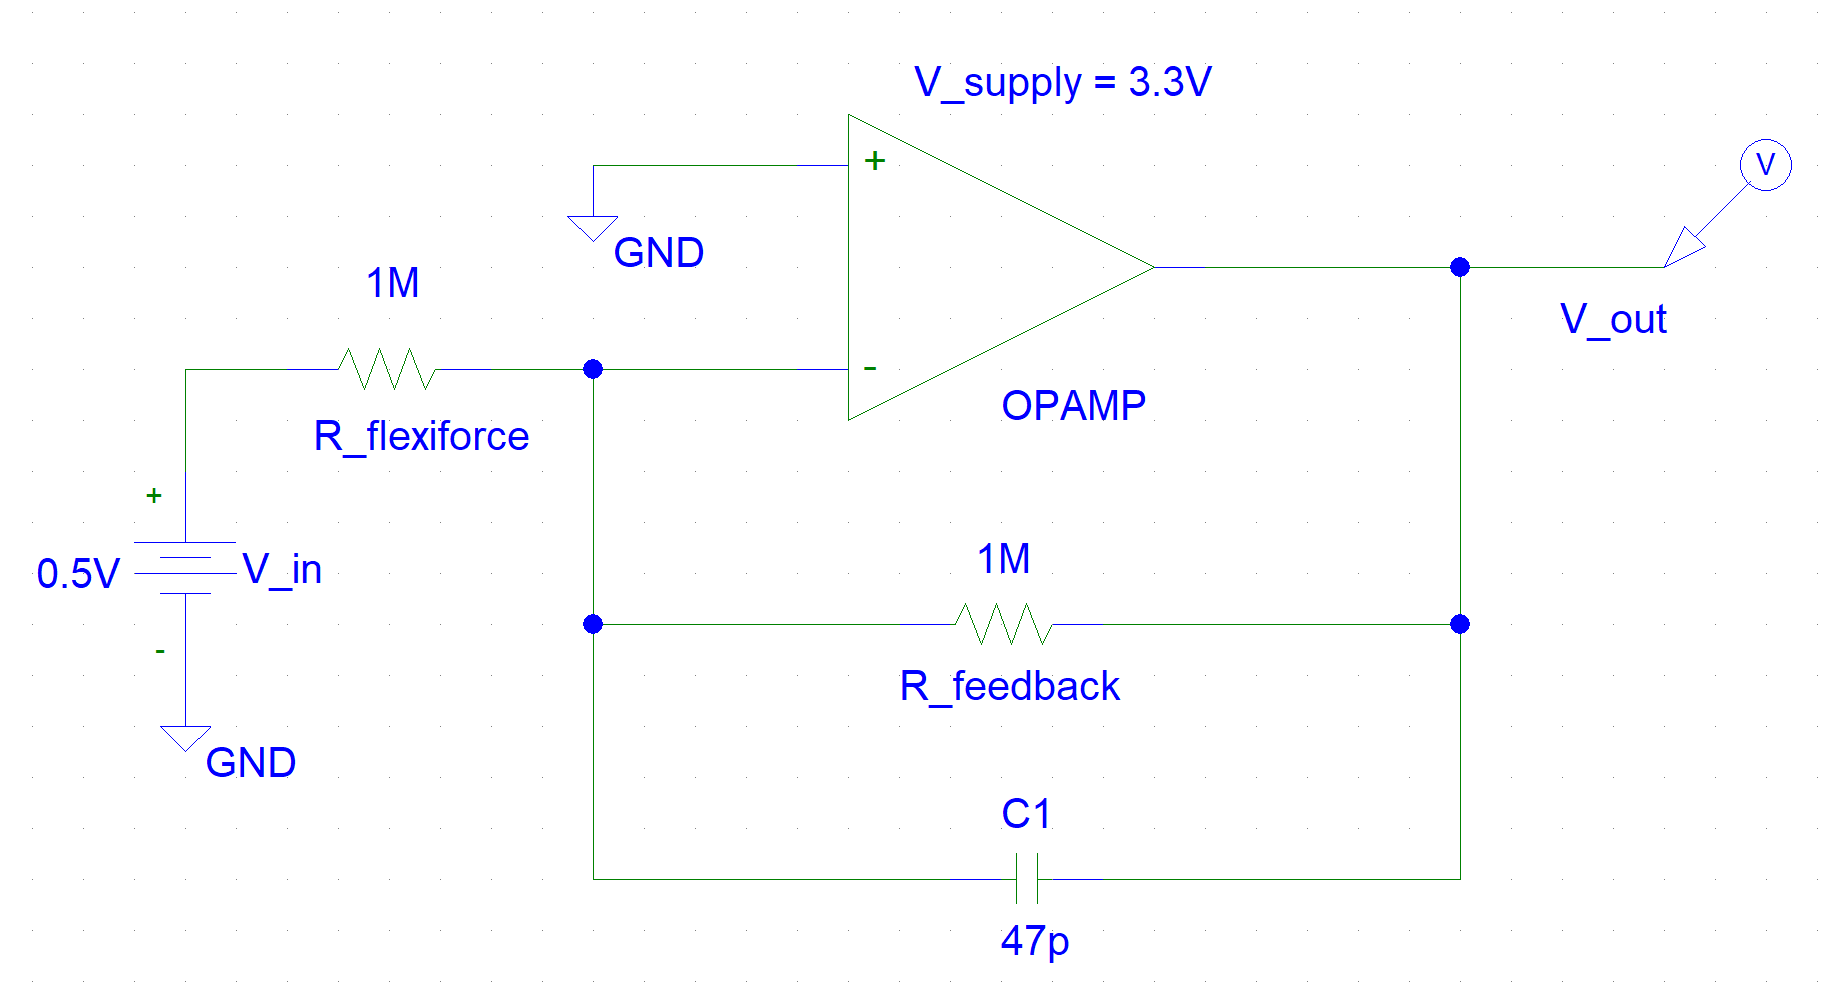
\includegraphics[width=.985\linewidth]{figures/capacitor.png}
    \caption{Inverting operational amplifier circuit with capacitor (created in PSpice)}
    \label{fig:capacitor}
\end{figure*}

\section{Simulating the circuits}
\label{sec:simulation}
The simulation of the alternative circuits was an important mean in designing and tuning the circuits. It was first and foremost important to look at the circuits behavior under ideal condition to understand how they would perform, in terms of output voltage. By simulation, the appropriate resistance values for resistors could be found. PSpice was the first simulation program for initial tests of functionality, were LTSpice was later used for 
\subsection{LTSpice}
\label{subsec:ltspice}

\subsection{PSpice}
\label{subsec:pspice}


\section{Chapter results}
\label{sec:circuitresults}

Several tests on the two circuits were conducted using an Arduino UNO microcontroller \ref{sec:arduinouno}. Each test consisted of 1000 samples for each circuit. To investigate the differences in measurement quality and noise handling, the Flexiforce A201 sensor was loaded with $200g$ and $500g$ calibration weights (Figure \ref{fig:opamp_test200} \& \ref{fig:opamp_test500}).

\begin{figure}[!htb]
   \begin{minipage}{0.470\textwidth}
     \centering
     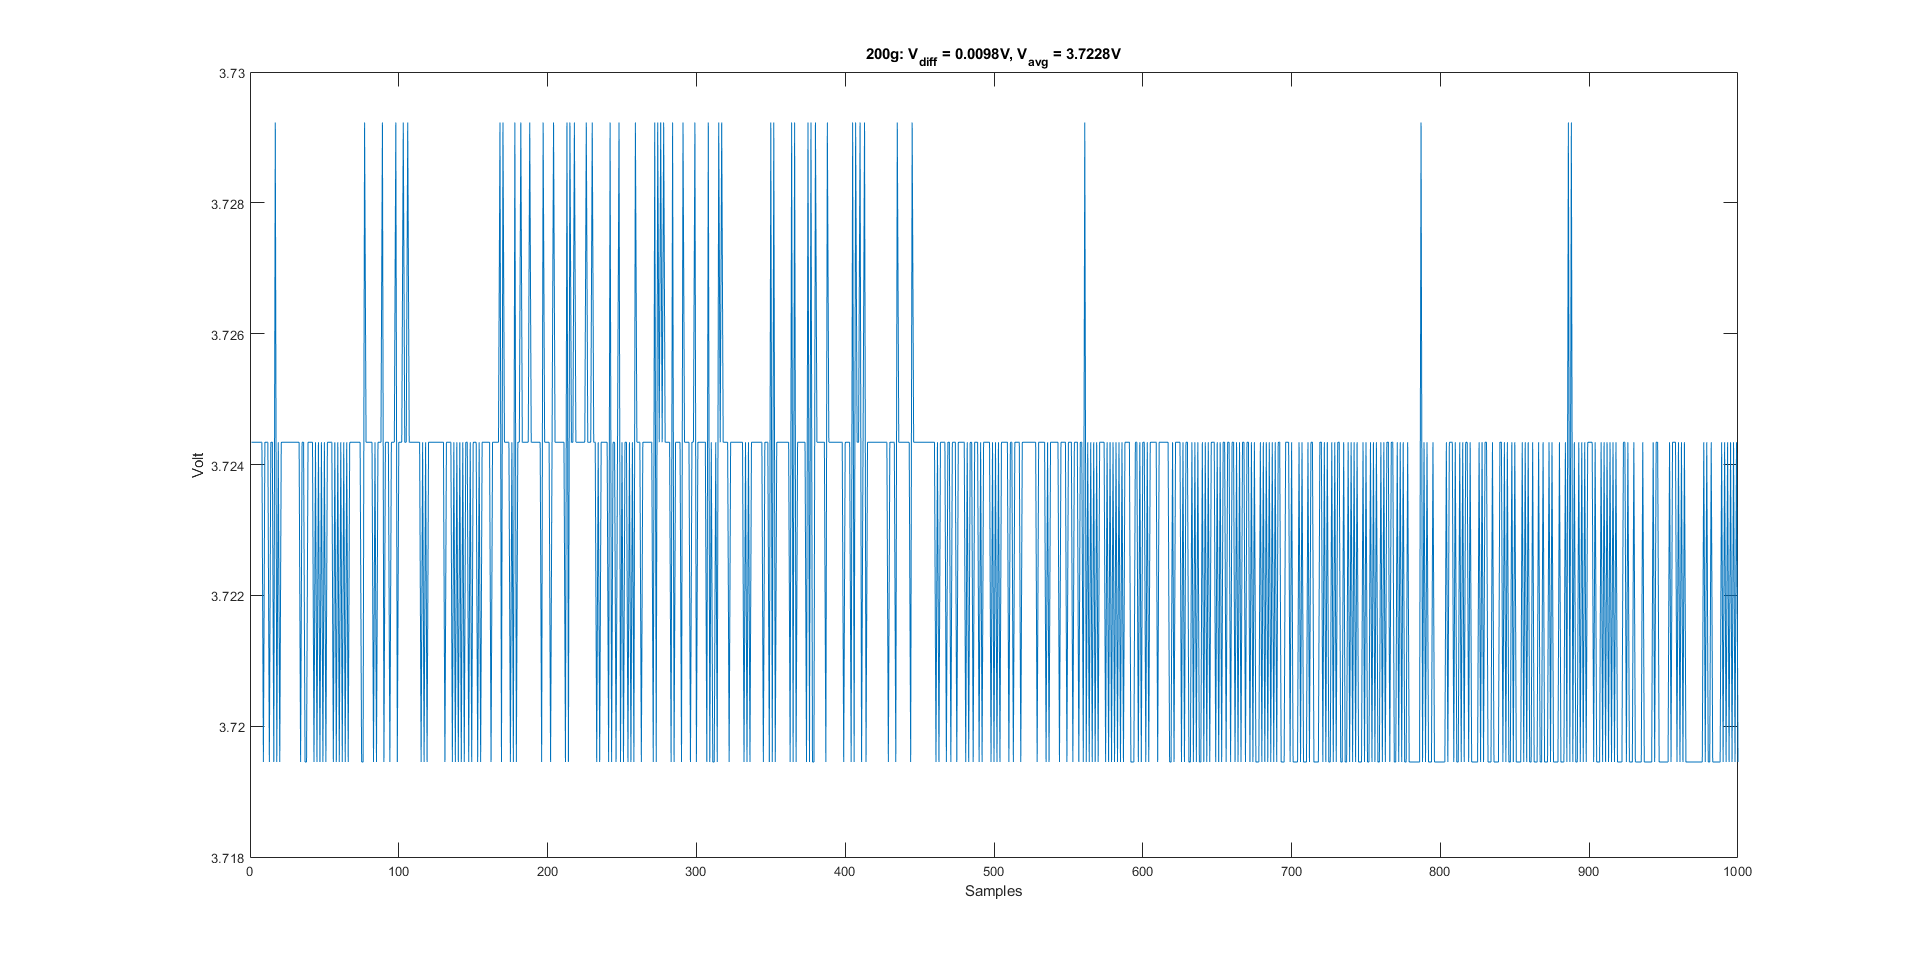
\includegraphics[width=0.7\textwidth]{figures/opamp_Vdiff_200g.png}
     \caption{1000 samples of 200g test for operational amplifier}
     \label{fig:opamp_test200}
   \end{minipage}\hfill
   \begin{minipage}{0.470\textwidth}
     \centering
     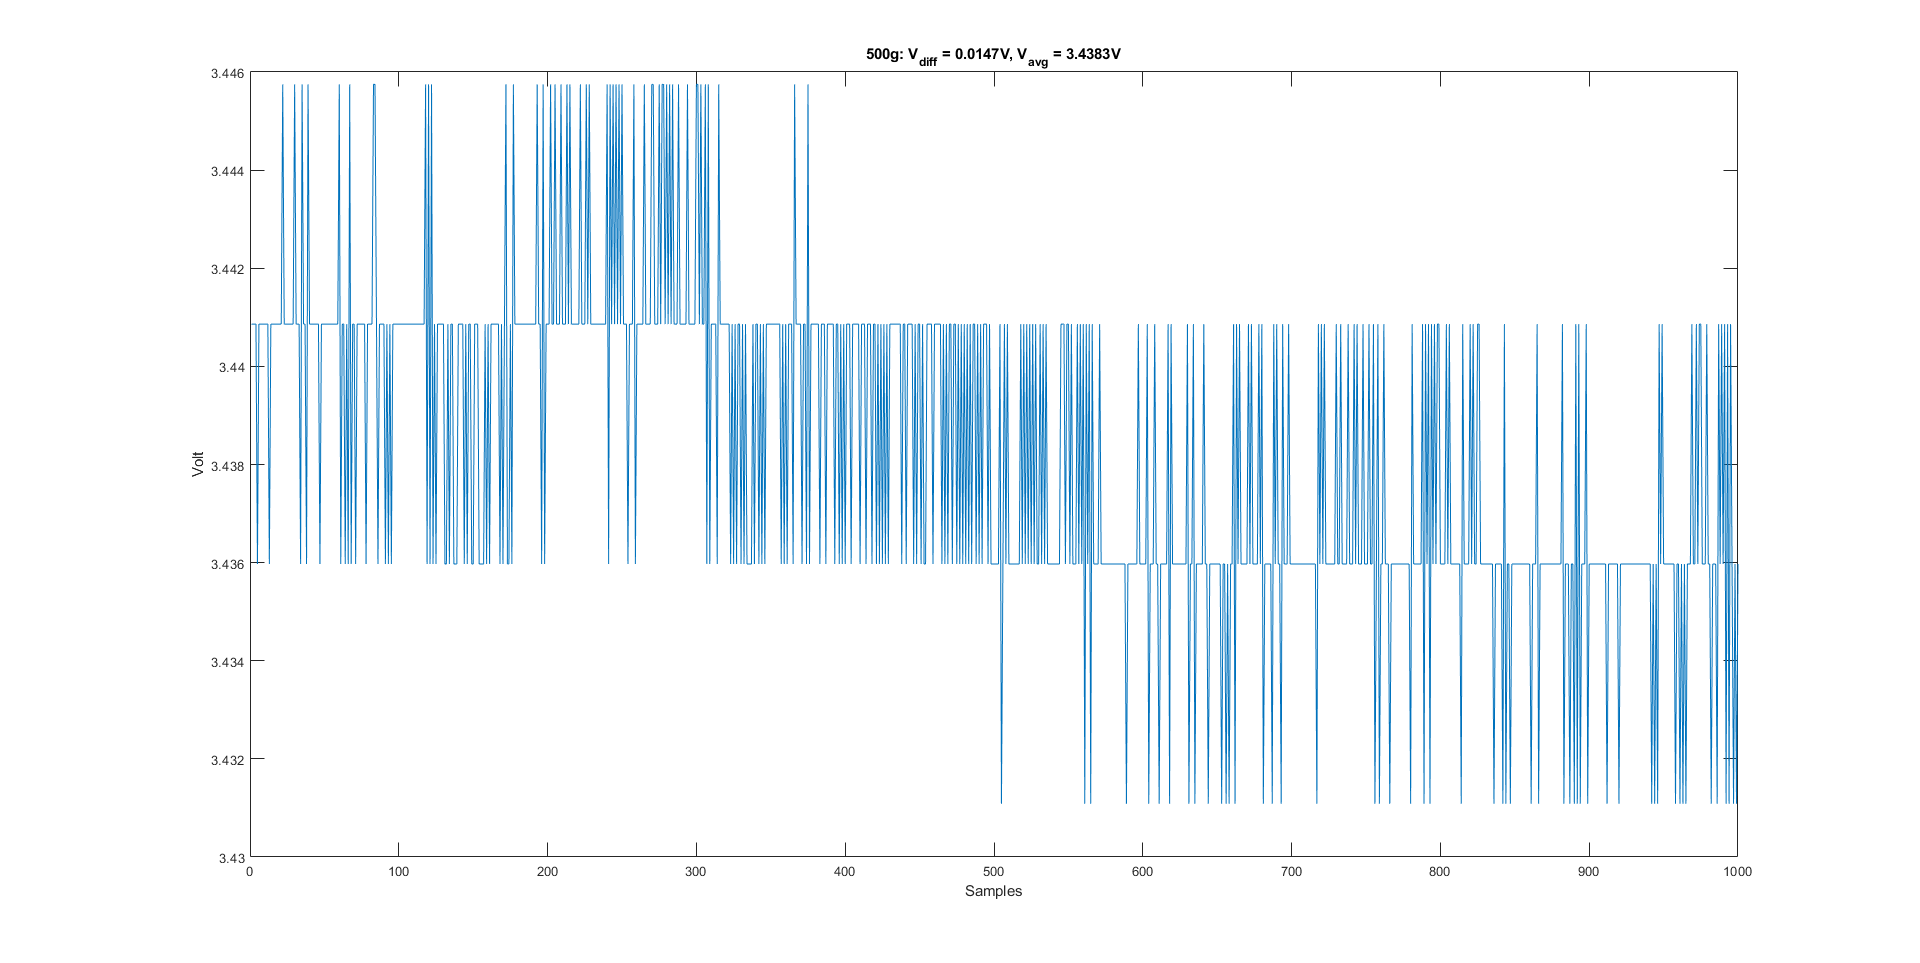
\includegraphics[width=0.7\textwidth]{figures/opamp_Vdiff_500g.png}
     \caption{500 sampling test for operational amplifier circuit with 500g weight, analysing voltage variation}
     \label{fig:opamp_test500}
   \end{minipage}
\end{figure}




\section{Chapter discussion}
\label{sec:circuitdisc}
In the process of selecting a force sensing sensor, it is required to chose the most suited sensor for the application area. In the research done by Fabrizio Vecchi and his colleagues \citep{vecchi_experimental_2000} on commercial sensors in biomechanics and motorcontrol, sensors like the \textit{Flexiforce A201 \ref{sec:flexiforce}} and \textit{Force Sensing Resistor \ref{sec:interlink}} were evaluated. In terms of linearity, time-drift tests and robustness, the Flexiforce sensor presented better results. As mentioned, the application area is what determines the choice of sensor, and for this thesis a sensor is required for handling forces significantly higher than the research conducted by Vecchi et. al (2000). The Flexiforce sensor in combination with the operational amplifier circuits prove to show similar results in terms of linearity, which is a key factor to obtain consistent and accurate results in measurements. After analysing the voltage divider and operational amplifier circuits, a clear difference in terms of noise and measurement spikes were observed. The operational amplifier circuit \ref{sec:opamps} proved to reduce the variation of voltage over time (Figur \ref{fig:opamp_test200} \& \ref{fig:opamp_test500}).


Needed weight to measure (45/4) osv.

\section{Summary}
\label{sec:circuitsummary}
Sensors and circuits presented in Section \ref{chap:sensors} and \ref{chap:circuits}, the linearity and consistency of measurements were tested and evaluated. Differences were found in terms of noise (measurement spikes and variance), linearity and precision. An operational amplifier circuit was selected reasoned by the requirement of precise measurements and linearity with low-noise outputs and low-power consumption. In combination with the Flexiforce A201 sensor, the system was able to handle the required forces up to 450\si{\newton} (or 45-46\si{\kilogram}). As suggested by Tekscan, Inc., a inverting operational amplifier circuit was chosen.
External and internal noise were handled by implementing a capacitor as a analog low pass filter, which proved to have a positive effect on the quality of the sampled data.
\begin{itemize}
    \item \textbf{!! How I calibrated and why}
\end{itemize}


\chapter{Digital measurements}
\label{chap:extracting}
\textit{\textbf{Chapter abstract:} summary of the chapter, start to finish}
\section{Microcontrollers}
\label{sec:microcontrollers}
Microcontrollers are small programmable computers used to control input and output gates. These gates are commonly used to control digital and analog circuits. A microcontrollers quality is measured by the capacity of the chip (processor) and the size of the analog-to-digital converters (ADC). The speed or capacity of the chip is measured in Hertz (Hz) and is the speed of how many operations the microcontroller can complete per second. The ADC is a component that converts a analog signals from a circuit to a digital signal on one or more of the input gates. The conversion is done by the ADC in a microcontroller with sample-and-hold techniques to produce a digital signal from the varying input. The quality of an ADC is measured in how many bits the ADC consists of. This translates to how many steps in the analog to digital conversion it is capable of. This is also referred to as the resolution. For example, an 8 bit ADC will have a resolution of $2^{8} = 256$ (Figure \ref{fig:adc}). Small errors in the conversions are unavoidable, thus choosing a higher bit ADC will always be more beneficial. A few microcontrollers are considered for the task of producing digital signals from circuits as mentioned in Section \ref{chap:sensors}.

\begin{figure*}[!b]
    \centering
    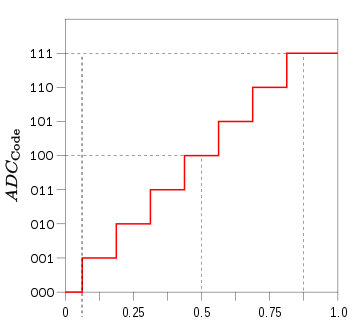
\includegraphics[width=0.49\textwidth]{figures/ADC_voltage_resolution.png}
    \caption{Concept of analog-to-digital conversion (Figure taken from \url{https://en.wikipedia.org/wiki/Analog-to-digital_converter})}
    \label{fig:adc}
\end{figure*}


\subsection{Raspberry Pi 3 Model A+}
1.4GHz Quad Core CPU, 512MB RAM, WiFi, BT, HDMI, MicroSD-card reader

\subsection{Arduino UNO Rev3}
\label{sec:arduinouno}
ATmega328P 16 MHz

\subsection{Arduino UNE}
Pros and cons, operating system, compatibility, ADC, sampling frequency, clock speed and ram.

\section{Software}
\label{sec:software}
This chapter gives and insight of which software was used

\subsection{Matlab}
\label{subsec:matlab}
What matlab is with pros and cons and how to generate plots.

\subsection{Arduino Software (IDE)}
The drivers used to read from the microcontroller

\section{Calibrating the system}
\label{sec:calibration}
The calibration of a pressure sensitive sensor can be done by calibrating the sensor at a minimum- and maximum-weight, adjusting the full-scale output. The output voltage is represented by forces loaded. This voltage can be calibrated and transformed directly to weight ($Kg$) for the specific sensor in use. Following, a line fit of the output full-scale can be created to make a system response of the system. This works well if we know the linearity of the measurements. If the conductance versus force linearity is known to increase more exponentially, we should consider using knots to section out certain parts of the full scale output.
\subsection{Calibration methods}
\label{subsec:calibrationmethods}
Calibration is an essential part of a measurement process and should be done regularly for consistent results. This section explains the concept of calibration why we do it.

\subsubsection{Modifying the full scale output}
The full scale output (FS) is the relation between input stimulus ($s$) and the output response. It defines the maximum value the system is able to output with given stimulus. Essentially, the full scale output is the measured voltage from the measurement system and can be modified digitally when reading the voltage.
The calibration method can typically be to create a system response based on a statistical line fitting model between a minimum- and maximum-value. For calibration in this thesis, we will see calibration be done with weights in five stages with different weights (also known as calibration knots). This is done by telling the system what weight has been loaded and referring this to the amount of voltage read by the micro controller (Chapter \ref{sec:microcontrollers}).

\subsection{Calibration weights}
For the sensors to be calibrated correctly, we are required to have a absolute scale of weights to refer our voltages to. This can be a certain amount of weights increasing linearly to the appropriate application area. For this thesis, a absolute scale can for example be from 1\si{\kilogram} to 20\si{\kilogram}.


\section{Chapter results}

\section{Chapter discussion}

\section{Summary}
\chapter{Discussion}
This chapter explains the results and analyses them.


\section{Mechanical properties}
How the mechanical properties can affect gliding speeds

\section{Pressure distribution}
What the pressure distribution means

\section{Span curve}
What the span curve means

\section{Friction affected by mechanical properties}
See if I can relate friction to the mechanical properties

\section{How to choose a ski}
\label{sec:choosingaski}
Looking into how we should choose a ski, we investigate the mechanical properties and how they relate to snow and weather conditions.
Choosing the correct ski for the ideal snow condition is based on the stiffness of the ski. For Classic skis, the choice of stiffness, $k$, to press the chamber height down to $0.2mm$ was around 66\% and 67\% of the body weight for men and women respectively and for warm conditions an increase to 77\% for both men and women.

Adjusting factors such as gliding wax and mechanical properties of the ski for different weather conditions and temperatures can result in better gliding speeds. In addition to these adjustable factors, a cold and warm condition is defined for each pair of skis. For temperatures below -3\textdegree C, skis for cold conditions are chosen. The skis for warm conditions typically are stiffer \citep{breitschadel_variation_2012}. We choose the ski with regard to stiffness to weight ratio for a given weather condition.



\chapter{Conclusion}
The aspect of pairing two skis with equal characteristics was considering in \citep{backstrom_essential_2008}, where the Swedish national team had been using a ski measurement device to measure the weight distribution for three years. As a result of these measurements, they had been able to measure all their skis and save the data for further matching of skis to the athletes. This is also an aspect that is interesting for this Master Thesis.

As a product of Felix Breitschädels research in 2013, a new test bench was developed to measure the chamber height and the span curves in individual skis to create a profile of the measured ski. This went under the category of a Finite Element Simulation to produce heat maps for the weight distribution. One of the problems discussed in the publication was the sensitivity of the model. The FE Simulation had the capability of producing good estimates of the span curve with given applied force $N$. The sensitivity mentioned was due to the inaccuracies in the measured deflection and the double derivative of the formula for calculating the bending stiffness:
\begin{equation}
    El = \frac{M}{k} , k \approx \frac{\partial^2 u}{\partial x^2} 
\end{equation}

\section{Further work}
What can be done in the future
\chapter{Conclusion}
As a product of Felix Breitschädels research in 2013, a new test bench was developed to measure the chamber height and the span curves in individual skis to create a profile of the measured ski. This went under the category of a Finite Element Simulation to produce heat maps for the weight distribution. One of the problems discussed in the publication was the sensitivity of the model. The FE Simulation had the capability of producing good estimates of the span curve with given applied force $N$. The sensitivity mentioned was due to the inaccuracies in the measured deflection and the double derivative of the formula for calculating the bending stiffness:
\begin{equation}
    El = \frac{M}{k} , k \approx \frac{\partial^2 u}{\partial x^2} 
\end{equation}

\section{Further work}
What can be done in the future
\begin{itemize}
    \item Different sensor, weight class below
    \item Different microcontroller with better ADC
    \item More linear calibration steps
    \item More accurate calibration process
    \item Upgrading the op-amp of the circuits for reduced amount of circuitboards
\end{itemize}

%\bibliographystyle{plainnat}
%\bibliography{mtbib}
\printbibliography
\begin{appendices}
\chapter{Matlab codes}
\section{calibration.m}
\section{readVoltage.m}

\end{appendices}

\end{document}
